\documentclass[a4paper,12pt]{article}

%%% Работа с русским языком

\usepackage{cmap}					% поиск в PDF
\usepackage{mathtext} 				% русские буквы в формулах
\usepackage[T2A]{fontenc}			% кодировка
\usepackage[utf8]{inputenc}			% кодировка исходного текста
\usepackage[english,russian]{babel}	% локализация и переносы
\usepackage{indentfirst}            % красная строка в первом абзаце
\usepackage[unicode]{hyperref}
\usepackage{epigraph}
\frenchspacing                      % равные пробелы между словами и предложениями

%%% Дополнительная работа с математикой
\usepackage{amsmath,amsfonts,amssymb,amsthm,mathtools} % пакеты AMS
\usepackage{bbm} % Blackboard bold для цифр
\usepackage{icomma}                                    % "Умная" запятая

\renewcommand{\phi}{\ensuremath{\varphi}}
\renewcommand{\kappa}{\ensuremath{\varkappa}}
\renewcommand{\le}{\ensuremath{\leqslant}}
\renewcommand{\leq}{\ensuremath{\leqslant}}
\renewcommand{\ge}{\ensuremath{\geqslant}}
\renewcommand{\geq}{\ensuremath{\geqslant}}
\renewcommand{\emptyset}{\ensuremath{\varnothing}}

\newcommand{\cl}{\text{cl }}
\newcommand{\setint}{\text{int }}
\newcommand\independent{\protect\mathpalette{\protect\independenT}{\perp}}
\def\independenT#1#2{\mathrel{\rlap{$#1#2$}\mkern2mu{#1#2}}}

\theoremstyle{plain}
\newtheorem{theorem}{Теорема}[section]
\newtheorem{lemma}{Лемма}[section]
\newtheorem{proposition}{Утверждение}[section]
\newtheorem*{corollary}{Следствие}
\newtheorem*{exercise}{Упражнение}

\theoremstyle{definition}
\newtheorem{definition}{Определение}[section]
\newtheorem*{note}{Замечание}
\newtheorem*{reminder}{Напоминание}
\newtheorem*{example}{Пример}
\newtheorem*{tasks}{Вопросы и задачи}

\theoremstyle{remark}
\newtheorem*{solution}{Решение}

%%% Оформление страницы
\usepackage{extsizes}     % Возможность сделать 14-й шрифт
\usepackage{geometry}     % Простой способ задавать поля
\usepackage{setspace}     % Интерлиньяж
\usepackage{enumitem}     % Настройка окружений itemize и enumerate
\usepackage{epigraph}     % Эпиграф
\setlist{leftmargin=25pt} % Отступы в itemize и enumerate

\geometry{top=25mm}    % Поля сверху страницы
\geometry{bottom=30mm} % Поля снизу страницы
\geometry{left=20mm}   % Поля слева страницы
\geometry{right=20mm}  % Поля справа страницы

\begin{document}
\tableofcontents
\newpage

\section{Комплексная дифференцируемость. Условия Коши-Римана}
\begin{definition}
	\textbf{Окрестностью} назовём
	\[
		B_r(z_0) = \{z \in \mathbb{C} \:\vert\: \vert z - z_0\vert < r\}
	\]
	\textbf{Проколотой окрестностью} назовём
	\[
		\dot{B}_r(z_0) = \{z \in \mathbb{C} \:\vert\: 0 < \vert z - z_0\vert < r\}
	\]
	\textbf{Замкнутой окрестностью} назовём
	\[
		\overline{B}_r(z) = \{z_0 \in \mathbb{C} \:\vert\: \vert z - z_0\vert \leq r\}
	\]
\end{definition}

\begin{note}
	Введём обозначения:
	\begin{align*}
		\Delta x := x - x_0 ;\;\;\;\; \Delta y := y - y_0 ;\;\;\;\; \Delta z := z - z_0 = \Delta x + i\Delta y \\
		\Delta u := u(x,\,y) - u(x_0,\,y_0);\;\;\; \Delta v := v(x,\,y) - v(x_0,\, y_0) ;\;\;\; \Delta f := f(x,\, y) - f(x_0,\, y_0) = \Delta u + i\Delta v
	\end{align*}
	где $f \equiv u + iv;\; u,\,v :\: \mathbb{R}^2 \to \mathbb{R}$.
\end{note}

\begin{definition}
	Говорят, что $f :\: B_r(z_0) \to \mathbb{C}$ \textbf{дифференцируема в точке} $z_0$, если
	\[
		\exists A \in \mathbb{C} :\: f(z) = f(z_0) + A(z - z_0) + o(z - z_0),\, \vert z - z_0\vert \to 0
	\]
\end{definition}

\begin{lemma}
	$f :\: B_r(z_0) \to \mathbb{C}$ дифференцируема в $z_0 \Leftrightarrow \exists f'(z_0),\, A = f'(z_0)$.
\end{lemma}

\begin{theorem}
	Условие Коши-Римана.

	$f :\: B_r(z_0) \to \mathbb{C}$ дифференцируема в $z_0$ тогда и только тогда, когда
	\begin{itemize}
		\item $u(x,\, y),\, v(x,\, y)$ дифференцируемы в $(x_0,\, y_0)$
		\item Выполняется условие Коши-Римана:
		      \[
			      \begin{cases}
				      \frac{\partial u}{\partial x} = \frac{\partial v}{\partial y} \\
				      \frac{\partial v}{\partial x} = -\frac{\partial u}{\partial y}
			      \end{cases}
		      \]
	\end{itemize}
	При этом
	\[
		f'(z_0) = \frac{\partial u}{\partial x}(x_0,\, y_0) + i\frac{\partial v}{\partial x}(x_0,\, y_0) = \frac{\partial v}{\partial y}(x_0,\, y_0) - i\frac{\partial u}{\partial y}(x_0,\, y_0)
	\]
\end{theorem}

\begin{proof}
	($\Rightarrow$)

	Пусть
	\[
		\exists f'(z_0) = a + ib = A \in \mathbb{C}
	\]
	Значит, по определению дифференцируемости
	\[
		\Delta f = A\Delta z + \alpha(\Delta z);\;\;\;\; \alpha(\Delta z) := \alpha_1(\Delta x,\, \Delta y) + i\alpha_2(\Delta x,\, \Delta y)
	\]
	Где $\alpha(\Delta z) = o(\Delta z),\, \vert\Delta z\vert \to 0$

	Тогда, раскрыв это выражение по каждой координате, получим
	\[
		\begin{cases}
			\Delta u = a\Delta x - b\Delta y + \alpha_1(\Delta x,\, \Delta y) \\
			\Delta v = b\Delta x + a \Delta y + \alpha_2(\Delta x,\, \Delta y)
		\end{cases}
	\]
	Из того, что $\vert\alpha_1\vert \leq \vert \alpha(\Delta z)\vert$ и $\vert\alpha_2\vert \leq \vert \alpha(\Delta z)\vert \Rightarrow \alpha_1,\, \alpha_2 = o(\Delta z),\, \vert \Delta z\vert \to 0$.

	Значит, $u$ дифференцируема, причём
	\[
		\frac{\partial u}{\partial x} = a ;\;\;\;\; \frac{\partial u}{\partial y} = -b
	\]
	Аналогично для $v$, причём
	\[
		\frac{\partial v}{\partial x} = b ;\;\;\;\; \frac{\partial v}{\partial y} = a
	\]
	Видим, что УКР выполняется.

	($\Leftarrow$)

	Пусть $u,\, v$ дифференцируемы в $(x_0,\, y_0)$ и выполняется УКР. Тогда
	\begin{align*}
		\Delta f = \Delta u + i\Delta v = \frac{\partial u}{\partial x}\Delta x + \frac{\partial u}{\partial y}\Delta y + \alpha_1(\Delta z) + i\left(\frac{\partial v}{\partial x}\Delta x + \frac{\partial v}{\partial y}\Delta y + \alpha_2(\Delta z)\right) = \\
		\Delta u + i\Delta v = \frac{\partial u}{\partial x}\Delta x - \frac{\partial v}{\partial x}\Delta y + \alpha_1(\Delta z) + i\left(\frac{\partial v}{\partial x}\Delta x + \frac{\partial u}{\partial x}\Delta y + \alpha_2(\Delta z)\right) =            \\
		\left(\frac{\partial u}{\partial x} + i\frac{\partial v}{\partial x}\right)\cdot(\Delta x + i\Delta y) + \alpha_1(\Delta z) + i\alpha_2(\Delta z)
	\end{align*}
	Значит,
	\[
		\exists f'(z_0) = \frac{\partial u}{\partial x} +i\frac{\partial v}{\partial x}
	\]
\end{proof}

\section{Связность. Теорема о голоморфной в области функции, производная которой равна нулю.}
\begin{definition}
	Множество $E \subseteq \overline{\mathbb{C}}$ называется \textbf{связным}, если не существует открытых $G_1,\, G_2$:
	\begin{enumerate}
		\item $G_1 \cup G_2 \supseteq E$
		\item $E \cap G_1 \cap G_2 = \emptyset$
		\item $E \cap G_1 \neq \emptyset$ и $E \cap G_2 \neq \emptyset$
	\end{enumerate}
\end{definition}

\begin{definition}
	Непустое открытое связное множество в $\overline{\mathbb{C}}$ называется \textbf{областью}.
\end{definition}

\begin{definition}
	Область $D$ называется \textbf{односвязной}, если $\overline{\mathbb{C}} \setminus D$ -- связно.
\end{definition}

\begin{definition}
	Функция $u :\: G \to \mathbb{R},\, G \subseteq \mathbb{R}^2$ -- область, причём
	\[
		u \in C^2(G),\, \Delta u = 0
	\]
	где $\Delta = \nabla^2 = \frac{\partial^2}{\partial x^2} + \frac{\partial^2}{\partial y^2}$, называется \textbf{гармонической}.
\end{definition}

\begin{definition}
	Функция $f :\: G \to \mathbb{C}$, где $G \subseteq \mathbb{C}$ -- область, называется \textbf{регулярной (голоморфной)}, если
	\[
		\forall z \in G \: \exists f'(z)
	\]
\end{definition}

\begin{definition}
	Функция $f :\: G \to \mathbb{C},\, G \subseteq \mathbb{C}$ называется \textbf{регулярной в точке} $z_0 \in G$, если
	\[
		\exists r > 0,\, B_r(z_0) \subseteq G :\: f \text{ регулярна на }B_r(z_0)
	\]
\end{definition}

\begin{theorem}
	Пусть $f$ голоморфна в области $D$ и
	\[
		\forall z \in D :\: f'(z) \equiv 0
	\]
	Тогда $f \equiv const$
\end{theorem}

\begin{proof}
	Любые $(x_0,\, y_0) \in D$ лежат вместе с каким-то отрезком $[(x_0,\, y_0),\, (x_0,\, y_0 + \Delta y)]$. Тогда
	\[
		f' = u_x + v_xi = v_y - u_yi \Rightarrow u_x \equiv v_x \equiv 0;\; u_y \equiv v_y \equiv 0
	\]
	Применим теорему Лагранжа к $u(x,\,y)$:
	\[
		\vert u(x_0,\, y_0 + \Delta u) - u(x_0,\, y_0)\vert = \Delta u\vert u'(x_0,\, \xi)\vert = 0 \Rightarrow u(x_0,\, y_0 + \Delta u) = u(x_0,\, y_0)
	\]
	Аналогично к $v(x,\,y) \Rightarrow f \equiv const$ на всех вертикальных отрезках.

	Аналогично на горизонтальных. Тогда $f \equiv const$ на $D$ в силу связности.
\end{proof}

\section{Теорема об обратной функции}
\begin{theorem}
	Пусть $f :\: G \to H \subseteq \mathbb{C},\, g :\: H \to \mathbb{C}$ регулярны. Тогда $\zeta(z) = g(f(z))$ также регулярна, причём
	\[
		\forall z \in G :\: \zeta'(z) = g'(f(z))f'(z)
	\]
\end{theorem}

\begin{proof}
	Зафиксируем $z_0 \in G,\, w_0 = f(z_0) \in G$.

	Из дифференцируемости
	\[
		\Delta f = f'(z_0)\Delta z + o(\Delta z),\, \vert\Delta z\vert \to 0;\;\;\;\; \Delta g = g'(w_0)\Delta w + o(\Delta w),\, \vert\Delta w\vert \to 0
	\]
	Пусть $\Delta w = \Delta f$, тогда
	\[
		\frac{\Delta\zeta}{\Delta z} = g'(w_0)\frac{\Delta f}{\Delta z} + \frac{o(\Delta f)}{\Delta f}\cdot\frac{\Delta f}{\Delta z} \overset{\Delta z \to 0}{\to} g'(w_0)f'(z_0) + 0
	\]
\end{proof}

\begin{theorem}
	Об обратной фнуции.

	Пусть $f :\: G \to \mathbb{C}$ регулярная и непрерывно дифференцируема на $G$. Пусть $z_0 \in G,\, w_0 = f(z_0),\, f'(z_0) \neq 0$. Тогда $\exists B_\delta(z_0),\, B_\varepsilon(w_0)$, такие, что
	\begin{enumerate}
		\item $\forall z \in B_\delta(z_0) :\: f'(z) \neq 0$
		\item $\forall \hat{w} \in B_\varepsilon(w_0)$ уравнение $\hat{w} = f(z)$ имеет в $B_\delta(z_0)$ единственное решение $\hat{z}$, то есть на $B_\varepsilon(w_0)$ определена обратная функция $g :\: B_\varepsilon(w_0) \to B_\delta(z_0)$, то есть
		      \[
			      \forall w \in B_\varepsilon(w_0) :\: f(g(w)) = w
		      \]
		\item $g$ регулярна на $B_\varepsilon(w_0)$, причём
		      \[
			      \forall w \in B_\varepsilon(w_0) :\: g'(w) = \frac{1}{f'(g(w))}
		      \]
	\end{enumerate}
\end{theorem}

\begin{proof}
	Первые два пункта выполняется благодаря обычной теореме об обратной функции из матана.

	Покажем, что мы имеем право применять ту самую теорему, для этого нам нужен ненулевой якобиан. Пусть $f(z) = u(x,\,y) + iv(x,\,y)$. Имеем отображение $\mathbb{R}^2 \to \mathbb{R}^2$. В силу непрерывной дифференцируемости этих двух функций запишем якобиан и преобразуем согласно УКР:
	\[
		J(x,\,y) = \begin{vmatrix}
			u_x & u_y \\
			v_x & v_y
		\end{vmatrix} = \begin{vmatrix}
			u_x & -v_x \\
			v_x & u_x
		\end{vmatrix} = (u_x)^2 + (v_x)^2 = \vert f'(z)\vert^2 \Rightarrow J(x_0,\, y_0) = \vert f'(z_0)\vert^2 \neq 0
	\]

	Третий пункт выполняется благодаря предыдущей теореме:
	\[
		g(f(z)) = z \Rightarrow g'(f(z))f'(z) = 1 \Rightarrow g'(f(z)) = \frac{1}{f'(z)} = g'(w) = \frac{1}{f'(g(w))}
	\]
\end{proof}

\section{Степенные ряды. Формула Коши-Адамара\dots}
\begin{definition}
	Ряд $\sum_{k = 1}^\infty g_k(z)$ сходится, если сходится последовательность $\{\sum_{k=1}^n g_k(z)\}_{n = 1}^\infty$.

	Сходимость бывает \textbf{условной} и \textbf{абсолютной} (когда сходится ряд из модулей).
\end{definition}

\begin{definition}
	\textbf{Степенным рядом} называется ряд вида
	\[
		\sum_{n = 0}^\infty a_nz^n,\, a_n \in \mathbb{C}
	\]
\end{definition}

\begin{theorem}
	Признак Вейерштрасса.

	Пусть
	\[
		\forall n \: \forall z:\: \vert g_n(z)\vert \leq \alpha_n
	\]
	причём $\sum_{n = 1}^\infty \alpha_n < +\infty$. Тогда ряд $\sum_{n = 1}^\infty g_n(z)$ сходится абсолютно равномерно.
\end{theorem}

\begin{theorem}
	Пусть $\frac{1}{R} := \overline{\lim}\sqrt[n]{\vert a_n\vert},\, R \in [0,\, +\infty]$. Тогда
	\begin{enumerate}
		\item Если $\vert z\vert \leq r < R$, то степенной ряд сходится равномерно и абсолютно.
		\item Если $\vert z\vert > R$, то ряд расходится
		\item $f(z) = \sum_{n = 0}^\infty a_nz^n$ голоморфна при $\vert z\vert < R$ и её производная получается почленным дифференцированием изначального ряда: $f'(z) = \sum_{n = 1}^\infty na_nz^{n-1}$
	\end{enumerate}
\end{theorem}

\begin{proof}
	\begin{enumerate}
		\item Пусть $\rho \in (r,\, R) \Rightarrow \frac{1}{R} < \frac{1}{\rho} < \frac{1}{r}$. По определению верхнего предела
		      \[
			      \exists N \in \mathbb{N} \: \forall n > N :\: \sqrt[n]{\vert a_n\vert} < \frac{1}{\rho}
		      \]
		      Тогда (в условиях текущего пункта):
		      \[
			      \exists N \in \mathbb{N} \: \forall n > N :\: \vert a_nz^n\vert \leq \left(\frac{r}{\rho}\right)^n,\, \frac{r}{\rho} < 1
		      \]
		      Тогда по теореме Вейшерштрасса мы можем ограничить рассматриваемый ряд сходящимся числовым (геометрическая прогрессия) и всё доказали.
		\item Пусть $\vert z\vert > R$, то есть $\frac{1}{\vert z\vert} < \frac{1}{R}$. Значит по плотности действительных чисел:
		      \[
			      \exists \varepsilon > 0 :\: \frac{1}{\vert z\vert} \leq \frac{1}{R} - \varepsilon \Rightarrow \vert z\vert \geq \frac{1}{\frac{1}{R} - \varepsilon}
		      \]
		      По определению верхнего предела:
		      \[
			      \exists \{n_k\}_{k = 1}^\infty \: \forall k :\: \sqrt[n_k]{\vert a_{n_k}\vert} > \frac{1}{R} - \varepsilon \Rightarrow \vert a_{n_k}z^{n_k}\vert \geq \left(\frac{1}{R} - \varepsilon\right)^{n_k}\cdot\left(\frac{1}{\frac{1}{R} - \varepsilon}\right)^{n_k} \geq 1
		      \]
		      Получили, что не выполнено необходимое условие сходимости ряда.
		\item Заметим, что у $g(z) = \sum_{n = 1}^\infty na_nz^{n-1}$ радиус сходимости такой же в силу $\sqrt[n]{n} \to 1$, то есть ряд сходится при $\vert z\vert < R$. Причём $\exists r :\: \vert z\vert \leq r < R$. Также введём обозначения:
		      \[
			      F_N(z) := \sum_{i = 0}^{N - 1} a_iz^i;\;\;\;\; H_N(z) := \sum_{i = N}^{+\infty} a_iz^i
		      \]

		      Заметим, что частичная сумма $G_n = F_n'$, то есть равна производной соответствующей частичной суммы $f$.

		      Распишем производную $f$ через частичные суммы:
		      \begin{align*}
			      \frac{f(z) - f(z_0)}{z - z_0} = \frac{F_N(z) - F_N(z_0)}{z - z_0} + \frac{H_N(z) - H_N(z_0)}{z - z_0} = \\
			      \left(\frac{F_N(z) - F_N(z_0)}{z - z_0}  - F_N'(z_0)\right) + (F_N'(z_0) - g(z_0)) + g(z_0) + \left(\frac{H_N(z) - H_N(z_0)}{z - z_0}\right)
		      \end{align*}
		      Устремляя $N \to +\infty$, получим
		      \[
			      \lim_{z \to z_0} \frac{f(z) - f(z_0)}{z - z_0} = g(z_0)
		      \]
		      так как
		      \[
			      \frac{H_N(z) - H_N(z_0)}{z - z_0} = \sum_{n = N}^\infty a_n\frac{z^n - z^n_0}{z - z_0} = \sum_{n = N}^\infty \left[a_n\sum_{k =0}^{n-1}z^kz_0^{n - 1 - k}\right] \Rightarrow
		      \]
		      \[
			      \left\vert\frac{H_N(z) - H_N(z_0)}{z - z_0}\right\vert \leq \sum_{n = N}^\infty \vert a_n\vert\cdot n\cdot r^{n - 1}
		      \]
		      Проследнее выражение стремится к нулю, как остаток сходящегося ряда.
	\end{enumerate}

\end{proof}

\section{Степенные ряды. Свойства экспоненты и тригонометрических.}
\begin{definition}
	Голоморфные в $\mathbb{C}$ функции называют \textbf{целыми}.
\end{definition}

\begin{definition}
	Определим эскпоненту
	\[
		e^z := \sum_{n = 0}^\infty \frac{z^n}{n!}
	\]
	$R_\text{сходимости} = +\infty \Rightarrow e^z$ целая.
\end{definition}

\begin{lemma}
	Свойства экспоненты:
	\begin{enumerate}
		\item $(e^z)' = e^z$
		\item $\forall z_1,\,z_2 \in \mathbb{C} :\: e^{z_1 + z_2} = e^{z_1}e^{z_2}$
		\item $\forall z \in \mathbb{C} :\: e^z \neq 0$
	\end{enumerate}
\end{lemma}

\begin{proof}
	\begin{enumerate}
		\item Сразу следует из пункта 3 предыдущей теоремы. (о почленном дифференцировании рядов)
		\item Покажем эквивалентное свойство $e^{a - z}e^z = e^a$. Пусть
		      \[
			      g(z) := e^{a - z}e^z \Rightarrow g'(z) = -e^{a - z}e^z + e^{a - z}e^z = 0
		      \]
		      А это значит, что $g \equiv const$, так как голоморфна.

		      Посчитаем $g(0) = e^{a - 0}e^0 = e^a \Rightarrow g(z) \equiv e^a$, что и требовалось доказать.
		\item $\forall z \in \mathbb{C}$ выполняется:
		      \[
			      e^ze^{-z} = e^0 = 1
		      \]
		      Значит в выражении $e^ze^{-z}$ никто не может быть нулём.
	\end{enumerate}
\end{proof}

\begin{definition}
	Определим тригонометрические функции на $\mathbb{C}$:
	\[
		\cos(z) := \sum_{n = 0}^\infty \frac{(-1)^nz^{2n}}{(2n)!} ;\;\;\;\; \sin(z) = \sum_{n = 0}^\infty \frac{(-1)^nz^{2n + 1}}{(2n + 1)!}
	\]
\end{definition}

\begin{lemma}
	Свойства тригонометрических функций:
	\begin{enumerate}
		\item $e^{iz} = \cos(z) + i\sin(z)$
		\item $\vert e^z\vert = e^{\text{Re}(z)}$
		\item Если $e^{z + T} = e^z$, то $T = 2\pi ik,\, k \in \mathbb{Z}$
	\end{enumerate}
\end{lemma}

\begin{proof}
	\begin{enumerate}
		\item Очевидно
		\item Очевидно
		\item Заметим, что
		      \[
			      e^T = 1 \Leftrightarrow \text{Re }T = 0 \Leftrightarrow T = i\beta
		      \]
		      Тогда
		      \[
			      e^{i\beta} = \cos(\beta) + i\sin(\beta) = 1 \Leftrightarrow \beta = 2\pi k \Rightarrow T = 2\pi ki,\, k \in \mathbb{Z}
		      \]
	\end{enumerate}
\end{proof}

\section{Первообразная и полный дифференциал в области. Условия\dots}
\begin{definition}
	\textbf{Кривой} $\gamma$ называется класс эквивалентных параметризаций (отличающихся лишь скоростью движения параметра)
	\[
		z(t) = x(t) + iy(t),\, t \in [t_0,\, t_1]
	\]
\end{definition}

\begin{definition}
	Кривая $\gamma$ называется \textbf{гладкой}, если существует параметризация
	\[
		z(t) = x(t) + iy(t),\, x,\, y \in C^1([t_0,\, t_1]);\;\; \forall t \in [t_0,\, t_1] :\: z'(t) \neq 0
	\]
\end{definition}

\begin{definition}
	Гладкая кривая $\gamma$ называется \textbf{замкнутой}, если
	\[
		z(t_0) = z(t_1);\;\; z'(t_0 + 0) = z'(t_1 - 0)
	\]
\end{definition}

\begin{definition}
	Кривая $\gamma$ называется \textbf{кусочно-гладкой}, если
	\[
		\exists\{\theta_i\}_{i = 0}^n :\: t_0 = \theta_0 < \theta_1 < \cdots < \theta_{n - 1} < \theta_n = t_1
	\]
	что
	\[
		\forall k = \overline{1,\,n} :\: \gamma|_{[\theta_{k - 1},\, \theta_k]} = z_k
	\]
	причём
	\[
		\forall k = \overline{1,\,n} :\: z_k(t),\, t \in [\theta_{k-1},\, \theta_k] \text{ - это гладкая кривая}
	\]
\end{definition}

\begin{definition}
	Пусть $g :\: G \to \mathbb{C}$, где $G$ -- область. Назовём $g$ \textbf{первообразной} непрерывной функции $f :\: G \to \mathbb{C}$, если $g$ регулярна на $G$ и
	\[
		\forall z \in G :\: g'(z) = f(z)
	\]
\end{definition}

\begin{definition}
	Выражение $f(z)dz$ называется \textbf{полным дифференциалом} в области $G$, если существует первообразная $g$ для $f$ на $G$, то есть
	\[
		f(z)dz = g'(z)dz
	\]
\end{definition}

\begin{theorem}
	Пусть $f :\: G \to \mathbb{C}$ непрерывна на области $G$. Тогда:
	\begin{enumerate}
		\item Если $fdz$ -- полный дифференциал на $G$, то для любой замкнутой КГК $\dot{\gamma} \subseteq G$ выполняется
		      \[
			      \int_{\dot{\gamma}}f(z)dz = 0
		      \]
		\item Если для любой замкнутой ломаной кривой $\gamma$ выполняется равенство выше, то $fdz$ -- полный дифференциал.
	\end{enumerate}
\end{theorem}

\begin{note}
	Первый пункт выполняется для всех КУСОЧНО-ГЛАДКИХ КРИВЫХ, второй же требует выполнение лишь для ЛОМАНЫХ (класс кривых гораздо меньше чем в первом пункте).
\end{note}

\begin{proof}
	\begin{enumerate}
		\item По условию $\exists g :\: G \to \mathbb{C}$, регулярная, такая, что $g'(z) = f(z)$. Тогда
		      \[
			      \int_{\dot{\gamma}}f(z)dz = \int_{t_0}^{t_1} g'(z(t))z'(t)dt = \int_{t_0}^{t_1}\frac{d}{dt}(g(z(t)))dt = g(z(t_1)) - g(z(t_0)) = g(z(t_0)) - g(z(t_0)) = 0
		      \]
		\item Фиксируем $a \in G$ как начальную точку ломаной $\gamma$. Тогда $\forall z \in G :\: \exists \gamma_{az}$ -- ломаная с началом в $a$ и концом в $z$.
		      \[
			      g(z) = \int_{\gamma_{az}} f(z)dz
		      \]
		      причём хотим показать, что этот интеграл не зависит от $\gamma_{az}$, а лишь от $z$.

		      Действительно, если $\exists \gamma_{az} \not\sim \tilde{\gamma}_{az}$, то пусть $\dot{\gamma} = \gamma_{az} \cup \tilde{\gamma}_{az}^{-1}$, тогда по аддитивности интеграла
		      \[
			      \int_{\dot{\gamma}}f(z)dz = 0 = \int_{\gamma_{az}}f(z)dz - \int_{\tilde{\gamma}_{az}}f(z)dz
		      \]
		      Докажем, что $\forall z :\: g'(z) = f(z)$. Рассмотрим $z_0 :\: \exists \varepsilon > 0 :\: B_\varepsilon(z_0) \subseteq G$ и приращение $\Delta z :\: 0 < \vert\Delta z\vert < \varepsilon$. Тогда $z_0 + \Delta z \in G$. Рассмотрим
		      \[
			      \frac{g(z_0 + \Delta z) - g(z_0)}{\Delta z} = \frac{1}{\Delta z} \int_{[z_0,\, z_0 + \Delta z]}f(z)dz
		      \]
		      Значит
		      \[
			      \left\vert\frac{\Delta g}{\Delta z} - f(z_0)\right\vert = \left\vert \frac{1}{\Delta z}\int_{[z_0,\, z_0 + \Delta z]}(f(z) - f(z_0)) dz\right\vert
		      \]
		      В силу непрерывности $f(z)$, найдём $r(\varepsilon)$ -- радиус шара, где $\vert f(z) - f(z_0)\vert < \varepsilon$, тогда
		      \[
			      \forall z \in B_{r(\varepsilon)}(z_0) \cap B_\varepsilon(z_0) :\: \left\vert \frac{\Delta g}{\Delta z} - f(z_0)\right\vert \leq \left\vert \frac{\varepsilon\min\{r(\varepsilon),\, \varepsilon\}}{\min\{r(\varepsilon),\, \varepsilon\}}\right\vert = \varepsilon
		      \]
	\end{enumerate}
\end{proof}

\section{Лемма Гурса и теорема Коши для выпуклой области}
\begin{lemma}
	Гурса.

	Пусть $G$ -- область, $f :\: G \to \mathbb{C}$ регулярна. Тогда для любого треугольника из $G$ (то есть такого, что $\partial\triangle \subseteq G$) верно
	\[
		\int_{\partial\triangle} f(z)dz = 0
	\]
\end{lemma}

\begin{proof}
	Зафиксируем $\triangle ABC \subseteq G$. Тогда будем рассматривать
	\[
		I := \int_{\partial\triangle ABC}f(z)dz
	\]
	Разобьём треугольник средними линиями:
	\[
		\triangle ABC = \bigcup_{k = 1}^4 \triangle_k
	\]
	Тогда из аддитивности интеграла
	\[
		I = \sum_{k = 1}^4 \int_{\partial \triangle_k}f(z)dz
	\]
	Докажем, что
	\[
		\exists k_0 :\: \left\vert \int_{\partial \triangle_{k_0}}f(z)dz\right\vert \geq \frac{\vert I\vert}{4}
	\]
	Очевидно от противного, так как триангуляции с ориентацией, то если бы все были меньше, то нельзя было бы набрать $I$.

	Обозначим найдённый треугольник за $\triangle^1 := \triangle_{k_0}$, а $\triangle^0 := \triangle ABC$. Аналогично построению $\triangle^1$ из $\triangle^0$ можем построить бесконечную последовательность $\{\triangle^N\}_{N = 0}^\infty$, и для них
	\[
		\left\vert \int_{\partial \triangle^N}f(z)dz\right\vert \geq \frac{\vert I\vert}{4^N}
	\]
	Теперь заметим, что $P_N = \frac{P_0}{2^N}$, где $P_N$ -- периметр $N$-го треугольника. В силу компактности
	\[
		\exists z_0 \in \bigcap_{N = 1}^\infty \triangle^N
	\]
	Так как $f$ дифференцируема в $z_0$, то по определению:
	\[
		\exists B_{\delta_0}(z_0) \: \forall z \in B_{\delta_0}(z_0) :\: f(z) = f(z_0) + f'(z_0)(z - z_0) + o(z - z_0)
	\]
	А для $o$-малого верно:
	\[
		\forall \varepsilon > 0 \: \exists \delta_1 \leq \delta_0 \: \forall z \in B_{\delta_1}(z_0) :\: \vert o(z - z_0)\vert \leq \varepsilon\vert z - z_0\vert
	\]
	Теперь можем расписать интеграл:
	\begin{align*}
		\int_{\partial\triangle^N}f(z)dz = f(z_0)\int_{\partial\triangle^N}dz + f'(z_0)\int_{\partial\triangle^N}zdz - z_0f'(z_0)\int_{\partial\triangle^N} dz + \int_{\partial\triangle^N}o(z - z_0)dz = \\
		\int_{\partial\triangle^N}o(z - z_0)dz
	\end{align*}
	Интегралы по $1$ и $z$ равны нулю, так как они, очевидно, полные дифференциалы.

	Причём полагаем $N$ таким, что
	\[
		\forall z \in \triangle^N :\: \vert z - z_0\vert < \delta_1
	\]
	Тогда
	\[
		\left\vert\int_{\partial\triangle^N} f(z)dz\right\vert \leq \int_{\partial\triangle^N} \vert o(z - z_0)\vert\cdot\vert dz\vert \leq \varepsilon\int_{\partial\triangle^N} \vert z - z_0\vert\cdot\vert dz\vert \leq \varepsilon P_N^2 \leq \varepsilon\frac{P_0^2}{4^N}
	\]
	Получили, что
	\[
		\vert I\vert \leq 4^N\left\vert\int_{\partial\triangle^N} f(z)dz\right\vert \leq 4^N\varepsilon\frac{P_0^2}{4^N}
	\]
	В силу произвольности $\varepsilon$: $I = 0$.
\end{proof}

\begin{theorem}
	Коши для выпуклой области.

	Пусть $D$ -- выпуклая область, $f$ -- голоморфна в $D \setminus \{0\}$, $f$ -- непрерывна в $D$. Тогда $\forall \gamma$ -- кусочно-гладкой замкнутой кривой
	\[
		\int_\gamma fdz = 0
	\]
\end{theorem}

\begin{proof}
	По лемме Гурса
	\[
		\forall \triangle \subseteq D :\: \int_{\partial \triangle} fdz = 0
	\]

	Тогда мы можем триангулировать любую ломаную (в силу выпуклости) $\Rightarrow$ по одной из теорем $fdz$ -- полный дифференциал (нужны были непрерывность и нулевой интеграл по всем ломаным).

	А как мы знаем, интеграл по любой замкнутой кривой от полного дифференциала нулевой.
\end{proof}

\section{Интеграл Коши и его свойства}
\begin{definition}
	Пусть $\gamma$ -- кусочно-гладкая кривая в $\mathbb{C}$. Тогда $\forall \phi \in C(\gamma)$ (непрерывная на $\gamma$ функции) определим \textbf{интеграл Коши}, как
	\[
		F_n(z,\, \phi) = \int_\gamma \frac{\phi(\xi)}{(\xi - z)^n}d\xi
	\]
\end{definition}

\begin{theorem}
	Свойства интеграла Коши:
	\begin{enumerate}
		\item $F_n(z,\, \phi)$ - голоморфна ($\Rightarrow$ непрерывна) в $\mathbb{C} \setminus \gamma$
		\item $F_n'(z,\, \phi) = nF_{n + 1}(z,\, \phi)$
	\end{enumerate}
\end{theorem}

\begin{proof}
	Вначале покажем непрерывность для $n = 1$:
	\[
		F_1(z,\, \phi) - F_1(z_0,\, \phi) = \int_\gamma\frac{\phi(\xi)(z - z_0)}{(\xi - z)(\xi - z_0)}d\xi = (z - z_0)\cdot F_1\left(z,\, \frac{\phi(\xi)}{\xi - z_0}\right)
	\]
	Введём $\delta = \rho(z_0,\, \gamma)$. Для $z_0 \in \mathbb{C}\setminus \gamma$ оно, очевидно, не равно нулю.

	Тогда
	\[
		\left\vert (z - z_0)\cdot F_1\left(z,\, \frac{\phi(\xi)}{\xi - z_0}\right)\right\vert \leq \frac{const}{\delta^2}\vert z - z_0\vert
	\]
	что и гарантирует непрерывность.

	Из того же тождества
	\[
		\frac{F_1(z,\, \phi) - F_1(z_0,\, \phi)}{z - z_0} = F_1\left(z,\, \frac{\phi(\xi)}{\xi - z_0}\right) \overset{z \to z_0}{\to} F_1\left(z_0,\, \frac{\phi(\xi)}{\xi - z_0}\right) = F_2(z_0,\, \phi)
	\]
	Доказали голоморфность существованием производной.

	Далее по индукции: пусть $F_{n - 1}$ голоморфна в $D$:
	\[
		F_{n - 1}'(z,\, \phi) = (n - 1)F_n(z,\, \phi)
	\]
	Распишем приращение с помощью умного нуля:
	\begin{align*}
		F_n(z,\, \phi) - F_n(z_0,\, \phi) =                                                                                                                                                   \\
		\int_\gamma\left[\left(\frac{1}{(\xi - z)^n} - \frac{1}{(\xi - z)^{n - 1}(\xi - z_0)}\right) + \frac{1}{(\xi - z)^{n - 1}(\xi - z_0)} - \frac{1}{(\xi - z_0)^n}\right]\phi(\xi)d\xi = \\
		(z - z_0)\int_\gamma\frac{\phi(\xi)d\xi}{(\xi - z)^n(\xi - z_0)} + F_{n - 1}\left(z,\, \frac{\phi(\xi)}{\xi - z_0}\right) - F_{n-1}\left(z_0,\, \frac{\phi(\xi)}{\xi - z_0}\right)
	\end{align*}
	Сходимость к нулю первого слагаемого доказывается аналогично предыдущему пункту с непрерывностью, а последние два слагаемых дают приращение непрерывной функции, которое также стремится к нулю при $z \to z_0$.

	Поделим предыдущее выражение на $z - z_0$ и посчитаем производную:
	\begin{align*}
		\frac{F_n(z,\, \phi) - F_n(z_0,\, \phi)}{z - z_0} = \int_\gamma\frac{\phi(\xi)d\xi}{(\xi - z)^n(\xi - z_0)} + \frac{F_{n - 1}\left(z,\, \frac{\phi(\xi)}{\xi - z_0}\right) - F_{n-1}\left(z_0,\, \frac{\phi(\xi)}{\xi - z_0}\right)}{z - z_0} \overset{z \to z_0}{\to} \\
		F_n\left(z_0,\, \frac{\phi(\xi)}{\xi - z_0}\right) + F_{n - 1}'\left(z_0,\, \frac{\phi(\xi)}{\xi - z_0}\right) = F_n\left(z_0,\, \frac{\phi(\xi)}{\xi - z_0}\right) + (n-1)F_n\left(z_0,\, \frac{\phi(\xi)}{\xi - z_0}\right) =                                        \\
		n\cdot F_n\left(z_0,\, \frac{\phi(\xi)}{\xi - z_0}\right) = n\cdot F_{n + 1}(z_0,\, \phi)
	\end{align*}
	Таким образом, $F_n(z,\, \phi)$ -- бесконечно дифференцируемая.
\end{proof}

\section{Интегральная формула Коши для круга\dots}
\begin{theorem}
	Пусть $f$ -- голоморфна в области $D$, причём $\overline{O}_r(a) \subset D$. Тогда
	\[
		\forall z \in O_r(a) :\: f(z) = \frac{1}{2\pi i} \int_{\vert \xi - a\vert = r}\frac{f(\xi)}{\xi - z}d\xi
	\]
\end{theorem}

\begin{proof}
	Фиксируем $z \in O_r(a)$:
	\[
		g(\xi) = \begin{cases}
			\frac{f(\xi) - f(z)}{\xi - z},\, \xi \neq z \\
			f'(z),\, \xi = z
		\end{cases}
	\]
	$g(\xi)$ -- голоморфна в $O_r(a) \setminus \{z\}$ (как отношение голоморфных функций) и непрерывна в $O_r(a) \Rightarrow \forall \gamma_r$ -- замкнутого контура по теореме Коши:
	\[
		\int_{\gamma_r}g(\xi)d\xi = 0
	\]
	То есть
	\[
		\int_{\gamma_r}\frac{f(\xi) - f(z)}{\xi - z}d\xi = 0 \Leftrightarrow
		\int_{\gamma_r}\frac{f(\xi)d\xi}{\xi - z} = f(z)\left[\int_{\gamma_r}\frac{d\xi}{\xi - z} =: G(z)\right]
	\]
	$G(z)$ -- голоморфна в $O_r(a),\, G' = \int_{\gamma_r} \frac{d\xi}{(\xi - z)^2} \equiv 0 \Rightarrow G \equiv const \Rightarrow G(a) = 2\pi i \Rightarrow$
	\[
		f(z) = \frac{1}{2\pi i} \int_{\gamma_r}\frac{f(\xi)d\xi}{\xi - z}
	\]
\end{proof}

\begin{corollary}
	\begin{enumerate}
		\item $f$ -- голоморфна в $D \Rightarrow f$ -- интеграл Коши $\Rightarrow f'$ -- голоморфна в $D$.
		\item $f$ -- голоморфна в $D \Rightarrow \forall n \in \mathbb{N} :\: f^{(n)}$ -- голоморфна в $D$.
		\item В условии формулы Коши для круга:
		      \begin{equation}\label{nElem}
			      f^{(n)}(z) = \frac{n!}{2\pi i} \int_{\vert \xi - a\vert = r} \frac{f(\xi)d\xi}{(\xi - z)^{n + 1}}
		      \end{equation}
	\end{enumerate}
\end{corollary}

\section{Теорема Морера. Теорема о среднем.}
\begin{theorem}
	Мореры.

	Пусть $f$ -- непрерывна в области $D$ и
	\[
		\forall \overline{\triangle} \subseteq D :\: \int_{\partial \triangle} f(z)dz = 0
	\]
	Тогда $f$ -- голоморфна в $D$.
\end{theorem}

\begin{proof}
	Заметим, что $\overline{O}_r(a) \subseteq D$ -- выпукло, поэтому применяем лемму о триангуляции ломаной треугольниками:
	\[
		\forall z \in O_r(a) \: \exists F :\: F' = f
	\]
	В этом круге по одному из следствий $F$ голоморфна $\Rightarrow f$ -- голоморфна в $O_r(a)$.

	Это верно $\forall a \in D \Rightarrow f$ -- голоморфна в $D$.
\end{proof}

\begin{theorem}
	О среднем.

	Пусть $f$ -- голоморфна в $\overline{O}_r(a) \subseteq D$, тогда
	\[
		f(a) = \frac{1}{2\pi}\int_0^{2\pi}f(a + e^{i\theta}r)d\theta
	\]
\end{theorem}

\begin{proof}
	Пусть $\xi = a + re^{i\theta}$. Тогда
	\[
		f(a) = \frac{1}{2\pi i}\int_0^{2\pi}\frac{f(a + re^{i\theta})ire^{i\theta}d\theta}{re^{i\theta}} = \frac{1}{2\pi}\int_0^{2\pi}f(a + re^{i\theta})d\theta
	\]
\end{proof}

\section{Целые функции и теорема Луивилля}
\begin{definition}
	$f$ -- \textbf{целая}, если $f$ голоморфна в $\mathbb{C}$.
\end{definition}

\begin{theorem}\label{Lui}
	Луивилля.

	Если $f$ -- целая и
	\[
		\exists M,\,m,\,R \: \forall z,\, \vert z\vert > R :\: \vert f(z)\vert < M\cdot\vert z\vert^m
	\]
	Тогда $f(z)$ -- полином степени $\leq m$.
\end{theorem}

\begin{proof}
	Знаем, что
	\[
		\forall z \in \mathbb{C} :\: f(z) = \sum_{n = 0}^\infty c_nz^n,\, R_{\text{сх}} = \infty
	\]
	Тогда по (\ref{Taylor})
	\[
		c_n = \frac{1}{2\pi i}\oint_{\vert \xi\vert = \rho} \frac{f(\xi)d\xi}{\xi^{n + 1}}
	\]
	Оценим сверху
	\begin{align*}
		\vert c_n\vert \leq \frac{1}{2\pi}\int_{\vert \xi\vert = \rho} \frac{\vert f(\xi)\vert\vert d\xi\vert}{\vert\xi^{n + 1}\vert} \leq \frac{M}{2\pi}\int_{\vert \xi\vert = \rho}\frac{\vert \xi\vert^m}{\vert\xi\vert^{n + 1}}\vert d\xi\vert = \\
		\frac{M}{2\pi}\int_{\vert \xi\vert = \rho}\frac{1}{\vert \xi\vert^{n + 1 - m}}\vert d\xi\vert = \frac{M}{\rho^{n - m}} = M\rho^{m - n}
	\end{align*}
	При $n > m$:
	\[
		\vert c_n\vert \leq \frac{M}{\rho^{n - m}} \overset{\rho \to +\infty}{\to} 0 \Rightarrow \forall n > m :\: \vert c_n\vert = 0 \Rightarrow f(z) = \sum_{n = 0}^m c_nz^n
	\]
\end{proof}

\section{Ряд Тейлора и теорема единственности\dots}
\begin{theorem}\label{Taylor}
	Ряд Тейлора.

	Пусть $f$ -- голоморфна в $D,\, O_R(a) \subseteq D$. Тогда
	\[
		\forall z \in O_R(a) :\: f(z) = \sum_{n = 0}^\infty c_n(z - a)^n,\, c_n = \frac{f^{(n)}(a)}{n!}
	\]
\end{theorem}

\begin{proof}
	Пусть $r < R,\, f$ -- голоморфна в $\overline{O_r(a)} \Rightarrow$
	\[
		2\pi if(z) = \int_{\gamma_r}\frac{f(\xi)d\xi}{\xi - z}
	\]
	Тогда распишем
	\begin{align*}
		\frac{1}{\xi - z} = \frac{1}{(\xi - a) - (z - a)} = \frac{1}{\xi - a}\cdot\frac{1}{1 - \frac{z - a}{\xi - a}} \overset{\vert z - a\vert < \vert \xi - a\vert}{=} \\
		\frac{1}{\xi - a}\sum_{n = 0}^\infty \left(\frac{z - a}{\xi - a}\right)^n = \sum_{n = 0}^\infty \frac{(z - a)^n}{(\xi - a)^{n + 1}}
	\end{align*}
	Полученный ряд сходится равномерно, а значит можно умножить на $f(\xi)$ и почленно интегрировать
	\begin{align*}
		2\pi i f(z) = \sum_{n = 0}^\infty \int_{\gamma_r}\frac{f(\xi)d\xi}{(\xi - a)^{n + 1}}(z - a)^n = \sum_{n = 0}^\infty 2\pi i c_n(z - a)^n \Rightarrow f(z) = \sum_{n = 0}^\infty c_n(z - a)^n
	\end{align*}
	Причём по (\ref{nElem}):
	\[
		c_n = \frac{f^{(n)}(a)}{n!}
	\]
	В завершение скажем
	\[
		\forall z :\: \vert z - a\vert < R \: \exists r < R \: z \in O_r(a) \Rightarrow
	\]
	формула верна во всём $O_R(a)$.
\end{proof}

\begin{definition}
	Пусть $f \not\equiv 0$ -- голоморфна в $O_r(a),\, f(a) = 0$, тогда $m$ -- это \textbf{порядок нуля в точке} $a$. если
	\[
		\forall k = \overline{0,\, m - 1} :\: f^{(k)}(a) = 0,\, f^{(m)}(a) \neq 0
	\]
\end{definition}

\begin{proposition}
	$f$ имеет нуль порядка $m \Leftrightarrow \exists g(z)$ -- голоморфная в $O_r(a),\, g(a) \neq 0$:
	\[
		f(z) = (z - a)^m\cdot g(z)
	\]
\end{proposition}

\begin{proof}
	($\Rightarrow$)

	БОО $a = 0$. Тогда
	\[
		f(z) = \sum_{n = 0}^\infty c_nz^n = \sum_{n = m}^\infty c_nz^n = z^m \sum_{n = 0}^\infty c_{n + m}z^n
	\]
	Пусть $g(z) :=\sum_{n = 0}^\infty c_{n + m}z^n$, причём $g(0) \neq 0$, так как $c_m \neq 0$.

	($\Leftarrow$) Пусть $f(z) = (z - a)^mg(z)$. Дифференцируя получаем
	\[
		\forall k = \overline{0,\,m-1} :\: f^{(k)}(a) = 0,\, f^{(m)} \neq 0
	\]
\end{proof}

\begin{note}\label{nonZero}
	Пусть $f$ -- голоморфна в окрестности $a,\, f(a) = 0$. Тогда
	\[
		\exists \rho > 0 \: \forall z \: \vert z - a\vert \in (0,\, \rho) :\: f(z) \neq 0
	\]
\end{note}

\begin{proof}
	Очевидно следует из предыдущего утверждения.
\end{proof}

\begin{theorem}
	О единственности.

	Пусть $f$ и $g$ -- голоморфны в области $D,\, E \subseteq D$, причём в $D$ есть хотя бы одна предельная точка $E$. Тогда если
	\[
		\forall z \in E :\: f(z) = g(z)
	\]
	то
	\[
		\forall z \in D :\: f(z) = g(z)
	\]
\end{theorem}

\begin{proof}
	Пусть $h = f - g,\, a $ -- предельная точка $E,\, a \in D$. Тогда введём
	\[
		Z = \{z \in D \:\vert\: h(z) = 0\}
	\]
	Тогда по непрерывности $a \in Z$, причём $a$ -- предельная точка $Z \Rightarrow h(z) \equiv 0$ в окрестности $a$ (\ref{nonZero}).

	Пусть $G_1 := \text{int }Z$ -- открытое непустое, так как $a \in G_1$. Тогда если $G_2 := D \setminus G_1$ открытое, то из-за связности $D \Rightarrow G_2$ -- пустое, что доказывает теорему.

	Пусть $G_2$ неоткрыто. Пусть $z^* \in G_2$, причём $z^*$ -- предельная точка $G_1$. Тогда $\exists z_n \to z^*,\, z_n \in G_1$. Тогда $h(z_n) = 0 \overset{\text{непрерывность}}{\Rightarrow} h(z^*) = 0 \Rightarrow$ $z^* \in G_1$ -- противоречие.
\end{proof}

\section{Приращение аргумента вдоль кривой. Индекс точки\dots}
\begin{definition}
	Пусть $\gamma$ -- кусочно гладкая кривая в $D$,
	\[
		\Gamma = f(\gamma) = \{w = f(z(t)) \:\vert\: t \in [\alpha,\, \beta]\}
	\]
	Причём $\Gamma$ -- кусочно гладкая, $\Gamma \subseteq \mathbb{C}\setminus\{0\}$. Тогда приращением аргумента вдоль кривой называется
	\[
		\Delta_\Gamma w := \text{Im }\int_\Gamma\frac{dw}{w} = \text{Im }\int_\gamma\frac{f'(z)dz}{f(z)} =: \Delta_\gamma f
	\]
\end{definition}

\begin{lemma}
	Свойства приращения аргумента:
	\begin{enumerate}
		\item $\Delta_\gamma(c\cdot f) = \Delta_\gamma(f),\, c \neq 0$
		\item $\Delta_\gamma(f_1\cdot f_2) = \Delta_\gamma(f_1) + \Delta_\gamma(f_2)$
		\item $\Delta_\gamma\frac{1}{f} = -\Delta_\gamma f$
		\item $\Delta_{-\gamma}(f) = -\Delta_\gamma(f)$
	\end{enumerate}
\end{lemma}

\begin{proof}
	\begin{enumerate}
		\item Следует из второго пункта (приращение константы равно нулю)
		\item Для доказательство достаточно заметить
		      \[
			      \frac{(f_1f_2)'}{f_1f_2} = \frac{f_1'}{f_1} +
			      \frac{f_2'}{f_2}
		      \]
		      И воспользоваться линейностью интеграла.
		\item Очевидно из предыдущего пункта
		\item Очевидно
	\end{enumerate}
\end{proof}

\begin{definition}
	\textbf{Индексом} $a$ относительно кривой $\gamma$, где $\gamma$ -- кусочно гладкая замкнутая кривая в $\mathbb{C},\, a \in \mathbb{C} \setminus \gamma$, называется
	\[
		J_\gamma(a) = \frac{\Delta_\gamma(z - a)}{2\pi} \in \mathbb{Z}
	\]
	Иными словами, это количество оборотов кривой вокруг $a$.
\end{definition}

\begin{lemma}
	Пусть $\gamma$ -- замкнутая кусочно-гладкая кривая в $\mathbb{C}$. Тогда
	\begin{enumerate}
		\item $J_\gamma(z) \equiv const$ в каждой компоненте связности $\mathbb{C}\setminus\gamma$
		\item Если какая-то компонента содержит $\infty$, то $J_\gamma(z) \equiv 0$ в ней.
	\end{enumerate}
\end{lemma}

\begin{proof}
	Действительно,
	\[
		J_\gamma(a) = \frac{1}{2\pi i}\int_\gamma\frac{dz}{z - a}
	\]
	интеграл Коши $\Rightarrow$ голоморфна в $\mathbb{C} \setminus \gamma \Rightarrow$ непрерывна и, так как принимает только значения из $\mathbb{Z}$, постоянна в своих компонентах связности. Это следует из того, что
	\[
		J_\gamma'(z) = \frac{1}{2\pi i} \int_\gamma\frac{d\xi}{(\xi - z)^2} = 0 \Rightarrow J_\gamma(a) \equiv const \text{ в компоненте связности}
	\]
	Для неограниченной компоненты
	\[
		d(z) := \text{dist }(\gamma,\, z) = \min_{\zeta \in \gamma}\vert z - \zeta\vert > 0
	\]
	Тогда
	\[
		\vert J_\gamma(z)\vert = \left\vert\frac{1}{2\pi i}\int_\gamma\frac{d\xi}{\xi - z}\right\vert \leq \frac{1}{2\pi d(z)}\int_\gamma\vert d\xi\vert
	\]
	Но $d(z) \to \infty$ при $z \to \infty \Rightarrow J_\gamma(z) = 0$.
\end{proof}

\section{Общая форма теоремы Коши и интегральной формулы Коши\dots}
\begin{lemma}
	Общая теорема Коши.

	Пусть $D$ -- область в $\mathbb{C},\, f$ -- голоморфна в области $D$. Тогда
	\begin{enumerate}
		\item Функция
		      \[
			      g(\xi,\, z) := \begin{cases}
				      \frac{f(\xi) - f(z)}{\xi - z},\, \xi \neq z \\
				      f'(z),\, \xi = z
			      \end{cases}
		      \]
		      непрерывна в $D \times D$.
		\item $\forall$ кусочно гладкой $\gamma \subset D$:
		      \[
			      h(z) = \int_\gamma g(\xi,\, z)d\xi
		      \]
		      голоморфна в $D$.
	\end{enumerate}
\end{lemma}

\begin{proof}
	\begin{enumerate}
		\item При $\xi \neq z$ непрерывна как отношение непрерывных функций.

		      При $\xi = z$ зафиксируем $z_0 \in D$, по открытости $D \Rightarrow \exists \overline{O}_r(z_0) \subset D$. Тогда будем рассматривать сколь угодно близкие $z,\, \xi \in O_\varepsilon(z_0),\, \varepsilon < r$.

		      Распишем в этой окрестности ряд Тейлора для двух точек:
		      \begin{align*}
			      f(z) - f(z_0) = \sum_{n = 1}^\infty c_n(z - z_0)^n \\
			      f(\xi) - f(z_0) = \sum_{n = 1}^\infty c_n(\xi - z_0)^n
		      \end{align*}
		      Далее нам понадобится следующая оценка:
		      \begin{align*}
			      \left\vert\frac{(z - z_0)^n - (\xi - z_0)^n}{z - \xi = [(z - z_0) - (\xi - z_0)]}\right\vert = \left\vert\sum_{k = 0}^{n - 1}(z - z_0)^{n - 1 - k}(\xi - z_0)^k\right\vert \leq n\varepsilon^{n-1}
		      \end{align*}
		      Рассмотрим приращение
		      \begin{align*}
			      \vert g(z,\, \xi) - g(z_0,\, z_0)\vert = \vert g(z,\, \xi) - f'(z_0)\vert \overset{f'(z_0) = \frac{c_1(z - z_0)}{z - z_0}}{=} \left\vert\sum_{n = 2}^\infty c_n \frac{(z - z_0)^n - (\xi - z_0)^n}{z - \xi}\right\vert \leq \\
			      \sum_{n = 2}^\infty \vert c_n\vert\cdot n\cdot\varepsilon^{n - 1} \leq \varepsilon\sum_{n = 2}^\infty \vert c_n\vert\cdot n\cdot r^{n - 2} = \varepsilon M
		      \end{align*}
		      Где $M < \infty$ взяли из сходимости ряда Тейлора путём дифференцирования ($\exists R > r :\: O_R(z_0) \subseteq D \: \overline{O}_r(z_0) \subseteq D$).

		      Заметим, что мы доказали непрерывность, оценив приращение $g$.
		\item Видно, что $h$ -- непрерывна в $D$. Тогда для $\overline{\triangle} \subset D$:
		      \[
			      \int_{\partial\triangle} h(z)dz = \int_{\partial\triangle}\int_\gamma g(\xi,\,z)d\xi dz = \int_\gamma\int_{\partial\triangle}g(\xi,\,z)dzd\xi = 0
		      \]
		      Это верно, так как $g(\xi_0,\, \cdot)$ голоморфна в $D \setminus \{\xi_0\}$, непрерывна в $D \Rightarrow$ по лемме Гурса $\int_{\partial\triangle}g(\xi,\,z)dz = 0$.

		      В итоге можем применить теорему Морера, из которой будет следовать, что $h$ -- голоморфна.
	\end{enumerate}
\end{proof}

\begin{definition}
	Пусть $\gamma_1,\, \cdots,\, \gamma_n$ -- замкнутые кусочно гладкие кривые. Тогда
	\[
		\Gamma = k_1\gamma_1 + \cdots + k_n\gamma_n
	\]
	где $k_i \in \mathbb{Z}$ мы будем называть \textbf{циклом}.
\end{definition}

\begin{definition}
	Пусть цикл $\Gamma$ лежит в области $D$. Тогда говорят, что $\Gamma \sim 0 \mod D$ ($\Gamma$ \textbf{гомологично эквивалентна} 0 в открытой области $D$), если
	\[
		\forall a \in \mathbb{C} \setminus D :\: J_\Gamma(a) = 0
	\]
\end{definition}

\begin{theorem}
	Интегральная теорема Коши.

	Пусть $D$ -- область в $\mathbb{C},\, f$ -- голоморфна в $D$. Пусть $\Gamma$ -- цикл в $D$, причём $\Gamma \sim 0 \mod D$. Тогда
	\begin{enumerate}
		\item $\forall z \in D \setminus \Gamma :\: J_\Gamma(z)\cdot f(z) = \frac{1}{2\pi i}\int_\Gamma \frac{f(\xi)d\xi}{\xi - z}$
		\item $\int_\Gamma f(z) dz = 0$
	\end{enumerate}
\end{theorem}

\begin{proof}
	($1 \Rightarrow 2$)

	Применим $1$ к $\tilde{f}(z) = (z - a)f(z)$. Где $a \in \mathbb{C} \setminus \Gamma$, если $f(a)$ определена (или $a \in D \setminus \Gamma$).

	Тогда
	\begin{align*}
		0 = J_\Gamma(a)(a - a)f(a) = J_\Gamma(a)\cdot\tilde{f}(a) = \int_\Gamma\frac{\tilde{f}(\xi)d\xi}{\xi - a} = \int_\Gamma f(\xi)d\xi
	\end{align*}

	Докажем первый пункт.

	Введём
	\[
		G := \{z \in \mathbb{C} \setminus \Gamma \:\vert\: J_\Gamma(z) = 0\}
	\]
	-- открытое множество. Рассмотрим две функции
	\[
		2\pi i \cdot\tilde{h}(z) = \int_\Gamma\frac{f(\xi)d\xi}{\xi - z}
	\]
	-- голоморфна в $G$, как интеграл Коши.

	\[
		2\pi i\cdot h(z) = \int_\Gamma\frac{f(\xi) - f(z)}{\xi - z}d\xi
	\]
	-- голомофрна в $D$, как функция из второго пункта предыдущей теоремы.

	Заметим, что $\forall z \in G \cap D :\: h(z) = \tilde{h}(z)$, так как
	\[
		\tilde{h}(z) - h(z) = \frac{1}{2\pi i}\int_\Gamma \frac{f(z)d\xi}{\xi - z} = f(z)J_\Gamma(z) = 0
	\]
	Тогда введём новую функцию
	\[
		F(z) := \begin{cases}
			h(z),\, z \in D \\
			\tilde{h}(z),\, z \in \mathbb{C}\setminus D \subseteq G \text{ так как } \Gamma \sim 0 \mod D
		\end{cases}
	\]
	Получается, $F(z)$ -- голоморфна в $\mathbb{C}$. (В каждой из гладких областей они голоморфны, и совпадают на границе)

	Заметим, что
	\[
		\lim_{z \to \infty} F(z) = 0
	\]
	Так как
	\[
		\vert\tilde{h}(z)\vert \leq \frac{1}{2\pi}\int_\Gamma\frac{\max_\Gamma \vert f\vert\cdot\vert d\xi\vert}{d(z)} \overset{z \to \infty}{\to} 0
	\]
	Где, $d(z) = \text{dist }(z,\, \Gamma) \Rightarrow d(z) \to \infty$.

	Тогда по теореме Луивилля (\ref{Lui}):
	\[
		F(z) \equiv 0
	\]
	Тогда в $D \setminus \Gamma :\: h(z) = F(z) = 0$, то есть
	\begin{align*}
		f(z)\cdot\frac{1}{2\pi i}\int_{\Gamma}\frac{d\xi}{\xi - z} = \frac{1}{2\pi i}\int_\Gamma\frac{f(\xi)d\xi}{\xi - z} \Rightarrow \\
		f(z)\cdot J_\Gamma(z) =  \frac{1}{2\pi i}\int_\Gamma\frac{f(\xi)d\xi}{\xi - z}
	\end{align*}
\end{proof}

\begin{corollary}
	Для односвязной области.

	Пусть $D$ -- односвязная область, $f$ голоморфна в $D$, $\Gamma$ -- замкнутая кусочно гладкая кривая в $D$. Тогда
	\[
		\int_\Gamma f(z)dz = 0
	\]
\end{corollary}

\begin{proof}
	Заметим, что $\forall a \not\in D :\: J_\Gamma(a) = 0$, так как $a$ лежит в компоненте связности, содержащей $\infty \Rightarrow$ можем использовать интегральную теорему Коши.
\end{proof}

\begin{corollary}
	Коши для многосвязной области.

	Пусть область $D$ ограничена циклом $\Gamma,\, f$ голоморфна в области $D' \supset D$. Тогда
	\begin{enumerate}
		\item $\forall z \in D :\: f(z) = \frac{1}{2\pi i}\int_\Gamma\frac{f(\xi)d\xi}{\xi - z}$
		\item $\int_\Gamma f(z)dz = 0$
	\end{enumerate}
\end{corollary}

\begin{proof}
	Имеем $0$ оборотов вокруг $D'$, а также один оборот вокруг $D \Rightarrow J_\Gamma(z) = 1 \Rightarrow$ по предыдущей теореме верен первый пункт, а второй выводится аналогично.
\end{proof}

\section{Разложение голоморфной функции в ряд Лорана\dots}
\begin{theorem}
	Пусть $f$ голоморфна в $K := \{z \:\vert\: r < \vert z - a\vert < R\}$. Тогда
	\[
		\forall z \in K :\: f(z) = \sum_{n = -\infty}^{+\infty}c_n(z - a)^n
	\]
	где
	\[
		c_n = \frac{1}{2\pi i}\cdot\int_{\gamma_\rho}\frac{f(\xi)d\xi}{(\xi - a)^{n + 1}}
	\]
	где $\gamma_\rho$ -- положительно ориентированная окружность радиуса $\rho \in (r,\, R)$ с центром в точке $a$.
\end{theorem}

\begin{proof}
	Докажем, что интегральная формула для $c_n$ не зависит от $\rho$. Возьмём две окружности радиуса $\rho$ и $\rho'$.

	Пусть $\Gamma := \gamma_\rho - \gamma_{\rho'}$. Применим теорему Коши для многосвязной области к функции $\frac{f(\xi)}{(\xi - a)^{n + 1}}$ (голоморфной в $K \supset K_{(\rho,\,\rho')}$). Тогда
	\[
		\int_\Gamma\frac{f(\xi)d\xi}{(\xi - a)^{n + 1}} = 0 \Leftrightarrow \int_{\gamma_\rho}\frac{f(\xi)d\xi}{(\xi - a)^{n + 1}} = \int_{\gamma_{\rho'}}\frac{f(\xi)d\xi}{(\xi - a)^{n + 1}}
	\]
	Рассмотрим $r < r' < R' < R$. Тогда $\forall z \in K'_{(r',\, R')}$:
	\[
		f(z) = \frac{1}{2\pi i}\int_\Gamma\frac{f(\xi)d\xi}{\xi - z} = \frac{1}{2\pi i} \left(\int_{\gamma_{R'}}\frac{f(\xi)d\xi}{\xi - z} - \int_{\gamma_{r'}}\frac{f(\xi)d\xi}{\xi - z}\right) =: f_1(z) + f_2(z)
	\]
	Заметим, что
	\[
		f_1(z) = \int_{\gamma_{R'}}\frac{f(\xi)d\xi}{\xi - z}
	\]
	голоморфна в $O_{R'}(a) \Rightarrow$
	\[
		f_1(z) = \sum_{n = 0}^\infty c_n(z - a)^n
	\]
	где $c_n = \frac{f^{(n)}(a)}{n!}$.

	Осталось разложить $f_2$:
	\[
		\frac{1}{z - \xi} = \frac{1}{(z - a) - (\xi - a)} = \frac{1}{z - a} \cdot\frac{1}{1 - \frac{\xi - a}{z - a}} = \sum_{n = 0}^\infty \frac{(\xi - a)^n}{(z -a)^{n + 1}}
	\]
	при $\left\vert\frac{\xi - a}{z - a}\right\vert < 1$.

	Значит
	\[
		f_2(z) = \sum_{n = 0}^\infty \frac{1}{(z - a)^{n + 1}}\cdot\left[c_{-n - 1} := \frac{1}{2\pi i}\int_{\gamma_{r'}}f(\xi)(\xi - a)^nd\xi \right]
	\]
	Получается, разложили так, что от $r'$ и $R'$ коэффициенты $c_n$ не зависят.
\end{proof}

\begin{definition}
	Такие ряды называются \textbf{рядами Лорана} для голоморфной функции $f$.
\end{definition}

\begin{theorem}
	Теорема о единственности ряда Лорана.

	Если $f(z) = \sum_{n = -\infty}^{+\infty}c_n(z - a)^n$ при $z \in K$, то $f$ -- голоморфна в кольце $K$, причём
	\[
		c_n = \frac{1}{2\pi i}\cdot\int_{\gamma_\rho}\frac{f(\xi)d\xi}{(\xi - a)^{n + 1}}
	\]
\end{theorem}

\begin{proof}
	$f$ голоморфна как предел сходящегося ряда

	Проверим равенство коэффициентов. Вначале для $n = -1$
	\[
		\int_{\gamma_\rho} f(z)dz = \sum_{n = -\infty}^{+\infty} c_n\cdot\int_{\gamma_\rho}(z - a)^ndz = 2\pi i\cdot c_{-1}
	\]
	При $n \neq -1$ сводим к предыдущему случаю для функции $\frac{f(z)}{(z - a)^{n + 1}}$
\end{proof}

\section{Изолированные особые точки}
\begin{definition}
	\textbf{Изолированная особая точка} -- точка, в некоторой проколотой окрестности которой функция $f(z)$ однозначна и голоморфна, а в самой точке либо не задана, либо недифференцируема.
\end{definition}

\begin{definition}
	$a$ -- \textbf{устранимая} особая точка, если
	\[
		\exists A \in \mathbb{C} :\: \lim_{z \to a} f(z) = A
	\]
\end{definition}

\begin{definition}
	$a$ -- \textbf{полюс}, если
	\[
		\lim_{z \to a} f(z) = \infty
	\]
\end{definition}

\begin{definition}
	$a$ -- \textbf{существенная} особая точка, если
	\[
		\not\exists \lim_{z \to a}f(x)
	\]
\end{definition}

\begin{theorem}
	$a$ -- УОТ $\Leftrightarrow f$ ограниченна в $\dot{O}_\delta(a)$ для некоторого $\delta$.
\end{theorem}

\begin{proof}
	($\Rightarrow$) -- очевидно по определению предела.

	($\Leftarrow$)

	Положим $M_\rho(f) = \max_{\gamma_\rho}\vert f\vert$. Тогда
	\[
		\vert c_n\vert \leq \frac{1}{2\pi}\int_{\gamma_\rho} \frac{\vert f\vert\vert d\xi\vert}{\rho^{n + 1}} \leq \frac{M_\rho(f)}{2\pi\rho^{n + 1}}\int_{\gamma_\rho}\vert d\xi\vert = \frac{M_\rho(f)}{\rho^n},\, n \in \mathbb{Z}
	\]
	По условию $f$ ограничена в $\dot{O}_\delta(a) \Rightarrow$
	\[
		\exists M \: \forall z \in O_\delta(a) :\: \vert f\vert < M
	\]
	Тогда из неравенства для $\vert c_n\vert$ следует
	\[
		\forall \rho > 0,\, \rho < \delta \Rightarrow \forall n < 0 :\: \frac{1}{\rho^n} \overset{\rho \to 0}{\to} 0 \Rightarrow \forall n < 0 :\: c_n = 0
	\]
	Значит
	\[
		f(z) = \sum_{n = 0}^\infty c_n(z - a)^n
	\]
	она имеет предел в точке $a$, равный $c_0$.
\end{proof}

\begin{theorem}
	Пусть $a$ -- изолированная особая точка $f$. Тогда $a$ полюс $\Leftrightarrow$ конечное число коэффициентов в главной части ряда Лорана отличны от нуля.
\end{theorem}

\begin{proof}
	($\Leftarrow$)

	По условию
	\[
		f(z) = \frac{c_{-m}}{(z - a)^m} + \cdots + \frac{c_{-1}}{z -a} + h(z)
	\]
	где $h$ -- голоморфна в окрестности $a$.

	Значит $\phi(z) := f(z)(z - a)^m$ -- голоморфная в этой области, причём $\phi(a) = c_{-m} \neq 0 \Rightarrow$
	\[
		\lim_{z \to a}f(z) = \frac{\lim_{z \to a} f(z)(z - a)^m}{\lim_{z \to a} (z - a)^m} = \infty
	\]

	($\Rightarrow$)

	По условию
	\[
		\lim_{z \to a} f(z) = \infty \Rightarrow \lim_{z \to a}\frac{1}{f(z)} = 0 \Rightarrow
	\]
	функция $\frac{1}{f(x)}$ имеет в т.$a$ УОТ $\Rightarrow$ она голоморфна в окрестности $a$. При этом $\frac{1}{f} \neq 0 \Rightarrow$
	\[
		\frac{1}{f(z)} = (z - a)^mh(z),\, h(a) \neq 0 \Rightarrow f(z) = \frac{1}{(z - a)^m}\frac{1}{h(z)}
	\]
	Где $\frac{1}{h(z)}$ -- голоморфная в окрестности $a$ $\Rightarrow$ раскладывается в Тейлора.
\end{proof}

\begin{theorem}
	Сохоцкого.

	Пусть $f$ голоморфна в $\dot{O}(a),\, a$ -- СОТ. Тогда
	\[
		\forall A \in \overline{\mathbb{C}} \: \exists z_n \to a :\: f(z_n) \to A
	\]
\end{theorem}

\begin{proof}
	\begin{enumerate}
		\item Для $A = \infty$ очевидно -- если $A$ -- не предельная, то $f$ ограничена $\Rightarrow a$ -- УОТ.
		\item Если $A \neq \infty$, то введём
		      \[
			      g(z) := \frac{1}{f(z) - A}
		      \]
		      Пусть $A$ -- не предельная. Тогда
		      \[
			      \exists \varepsilon > 0 \: \exists \delta > 0 \: \forall z \in \dot{O}_\delta(a) :\: \vert f(z) - A\vert \geq \varepsilon
		      \]
		      Значит $g(z)$ голоморфна в $\dot{O}_\delta(a)$ как отношение голоморфных функций. Причём $g(z) \neq 0$ в $\dot{O}_\delta(a)$. Также $\vert g(z)\vert \leq \frac{1}{\varepsilon} \Rightarrow g$ -- ограниченная, то есть точка $a$ -- УОТ. Тогда
		      \[
			      \forall z \in \dot{O}_\delta(a) :\: f(z) = A + \frac{1}{g(z)}
		      \]
		      Если $g(a) \neq 0$, то $a$ -- УОТ для $f$.

		      Если $g(a) = 0 \Rightarrow \frac{1}{g(z)}$ имеет полюс в точке $a \Rightarrow$ у $f$ точка $a$ -- полюс. Противоречие.
	\end{enumerate}
\end{proof}

\section{Вычеты и формулы для их вычисления. Теорема Коши о вычетах.}
\begin{definition}
	Если $f$ голоморфна в $\dot{O}_r(a),\, a \neq \infty$, то определим \textbf{вычет} $f$, как
	\[
		\text{res}_af = \frac{1}{2\pi i}\int_{\gamma_\rho}f(z)dz
	\]
\end{definition}

\begin{proposition}
	Вычеты определены корректно (независят от $\gamma$).
\end{proposition}

\begin{proof}
	Если $f(z) = \sum_{n = -\infty}^{+\infty} c_nz^n,\, z \in \dot{O}_r(a)$, то
	\begin{align*}
		\frac{1}{2\pi i}\int_{\gamma_\rho}f(z)dz = \sum_{n = -\infty}^{+\infty}\frac{1}{2\pi i}c_n\int_{\gamma_\rho}(z - a)^ndz = \frac{1}{2\pi i}c_{-1}2\pi i = c_{-1}
	\end{align*}
\end{proof}

\begin{theorem}
	Коши о вычетах.

	Пусть $D$ ограничена циклом $\Gamma = \gamma_0 - \gamma_1 - \cdots - \gamma_n$ (то есть в условиях теоремы Коши для многосвязной области).

	Пусть $A = \{a_1,\,\cdots,\, a_N\} \subseteq D,\, f$ -- голоморфна в $D' \setminus A$, где $D' \supseteq D$. Тогда
	\[
		\frac{1}{2\pi i}\int_\Gamma f(z)dz = \sum_{i = 1}^N \text{res}_{a_i} f
	\]
\end{theorem}

\begin{proof}
	Очевидно, что
	\[
		\exists R > 0 \: \forall i \neq j :\: \overline{O}_R(a_i) \cap \overline{O}_R(a_j) = \emptyset
	\]
	и $\overline{O}_R(a_i) \subseteq D$.

	Обозначим за обход $\delta_k = \partial O_R(a_k)$ (обход против часовой стрелки, то есть положительно ориентировано).

	Обозначим $\tilde{\Gamma} = \Gamma - \sum_{i = 1}^N \delta_i,\, \tilde{D} = D \setminus \cup_{k = 1}^N \overline{O}_R(a_k)$ и $\tilde{D}' = D'
		\setminus A$. Тогда $\partial\tilde{D} = \tilde{\Gamma}$ и $f$ голоморфна в $\tilde{D}'$.

	Причём $\tilde{D}' \supseteq \tilde{D}$. Более того, $\tilde{\Gamma} \sim 0 \: \mod \tilde{D}'$, и $\forall z \not\in \tilde{D}' :\: J_{\tilde{\Gamma}}(z) = 0$. Аналогично проверим для
	\begin{enumerate}
		\item $z \not\in D' \Rightarrow \begin{cases}
				      J_\Gamma(z) = 0 \\
				      J_{\delta_i}(z) = 0
			      \end{cases} \Rightarrow J_{\tilde{\Gamma}}(z) = 0$
		\item $z \in A \: (z = a_i) \Rightarrow \begin{cases}
				      J_{-\delta_i}(a_i) = -1              \\
				      J_{-\delta_j}(a_i) = 0 \: (i \neq j) \\
				      J_{\gamma_k}(a_i) = 0                \\
				      J_\Gamma(a_i) = 1
			      \end{cases} \Rightarrow J_{\tilde{\Gamma}}(z) = 0$
	\end{enumerate}
	Тогда по теореме Коши для многосвязной области $\tilde{D}$:
	\[
		\int_{\tilde{\Gamma}} f(z)dz = 0 \Rightarrow \sum_{i = 1}^N\int_{\delta_i}f(z)dz = \int_\Gamma f(z)dz \Rightarrow 2\pi i\sum_{i = 1}^N\text{res}_{a_i}(f) = \int_\Gamma f(z)dz
	\]
\end{proof}

\begin{corollary}
	Если $a$ -- УОТ $\Rightarrow \text{res}_af = 0$
\end{corollary}

\begin{corollary}
	Если $a$ -- полюс $m$-ого порядка $\Rightarrow$
	\[
		\text{res}_af = \frac{1}{(m - 1)!}\lim_{z \to a}\left(f(z)(z - a)^m\right)^{(m - 1)}
	\]
\end{corollary}

\begin{proof}
	$f$ имеет вид
	\[
		f = \sum_{n = -m}^\infty c_{n}(z - a)^n
	\]
	Тогда
	\[
		\text{res}_af = c_{-1} = \frac{1}{(m - 1)!}\lim_{z \to a}\left(f(z)(z - a)^m\right)^{(m - 1)}
	\]
	То есть по сути $m - 1$ коэффициент функции $f(z)(z - a)^m$.
\end{proof}

\section{Лемма Жордана.\dots}
\begin{theorem}
	Пусть $g$ -- непрерывная функция в $\{z \:\vert\: \text{Im}(z) \geq 0,\, \vert z\vert > R'\}$, причём $\max_{\Gamma_R}\vert g\vert \overset{R \to \infty}{\to} 0$, где $\Gamma_R = \{z \:\vert\: \text{Im}(z) \geq 0,\, \vert z\vert = R\}$. Тогда
	\[
		\forall \alpha > 0 :\: \int_{\Gamma_R} g(z)e^{i\alpha z}dz \to 0,\, R \to \infty
	\]
\end{theorem}

\begin{proof}
	Достаточно доказать, что $\int_{\Gamma_R}\vert e^{i\alpha z}\vert\vert dz\vert$ равномерно ограничен. (то есть $\exists M > 0 \: \forall R > R' :\: \int_{\Gamma_R}\vert e^{i\alpha z}\vert\vert dz\vert \leq M$).

	Пусть $z = Re^{i\phi},\, \phi \in (0,\, \pi)$, тогда очевидно,
	\[
		\vert e^{i\alpha z}\vert = e^{\text{Re}(i\alpha z)} = e^{-R\alpha\sin(\phi)}
	\]
	Теперь распишем интеграл
	\[
		\int_{\Gamma_R}\vert e^{i\alpha z}\vert\vert dz\vert = \int_0^\pi e^{-R\alpha\sin\phi}Rd\phi = 2R\int_0^{\frac{\pi}{2}}e^{-R\alpha\sin\phi}d\phi
	\]
	Вспомним, что $\sin\phi$ вогнут на $[0,\, \frac{\pi}{2}] \Rightarrow \sin\phi \geq \frac{2}{\pi}\phi$. Продолжим цепочку неравенств
	\begin{align*}
		2R\int_0^{\frac{\pi}{2}}e^{-R\alpha\sin\phi}d\phi \leq 2R\int_0^{\frac{\pi}{2}}e^{-\frac{2}{\pi}R\alpha\phi}d\phi = \frac{\pi}{\alpha}\int_0^{R\alpha}e^{-t}dt \leq \frac{\pi}{\alpha}\int_0^{+\infty}e^{-t}dt = \frac{\pi}{\alpha}
	\end{align*}
\end{proof}

\section{Принцип аргумента. Теорема Руше. Основная теорема алгебры.}
\begin{theorem}
	Принцип аргумента.

	Пусть $\Gamma = \gamma_0 - \gamma_1 - \cdots - \gamma_n,\, D$ -- область, ограниченная $\Gamma,\, A := \{a_1,\,\cdots,\, a_k\} \subseteq D,\, f$ голоморфна в $D' \setminus A,\, D' \supset D$. $a_j$ -- полюса функции $f$ и $\forall z \in \Gamma :\: f(z) \neq 0$. Тогда
	\[
		\frac{1}{2\pi i}\int_\Gamma\frac{f'}{f}dz = J_{f(\Gamma)}(0) = \frac{1}{2\pi}\Delta_\Gamma f = N - P
	\]
	где $N$ и $P$ -- число нулей и полюсов $f$ в $D$ с учётом их кратностей соответственно.
\end{theorem}

\begin{proof}
	Из определения $f$, можем её представить в виде
	\[
		f = \frac{(z - b_1)^{n_1}\cdots(z - b_\eta)^{n_\eta}}{(z - a_1)^{p_1}\cdots(z - a_k)^{p_k}}g(z)
	\]
	где $g$ -- голоморфна в $\overline{D}$ и не содержит там нулей.

	Тогда
	\[
		\frac{f'}{f} = \sum_{i = 1}^\eta\frac{n_i}{z - b_i} - \sum_{i = 1}^k\frac{p_i}{z - a_i} + \frac{g'}{g}
	\]
	Почему это так? Рассмотрим, например, $f(z) = (z - b_k)^{n_k}g(z)$, тогда $f'(z) = n_k(z - b_k)^{n_k - 1}g(z) + (z - b_k)^{n_k}g'(z)$. Тогда выполнено следующее:
	\[
		\frac{f'}{f} = \frac{n_k}{z - b_k} + \frac{g'}{g}
	\]
	Причём после интегрирования первое слагаемое даст нам приращение, а второе ноль, так как функция голоморфная. На случай нескольких нулей и полюсов обобщается аналогично.

	Значит
	\[
		\frac{1}{2\pi i} \int_\Gamma\frac{f'}{f}dz = \sum_{i = 1}^\eta n_iJ_\Gamma(b_i) - \sum_{i = 1}^k p_iJ_\Gamma(a_i) + \frac{1}{2\pi i}\int_\Gamma\frac{g'}{g}dz = \sum_{i = 1}^\eta n_i - \sum_{i = 1}^k p_i = N - P
	\]
	так как $J_\Gamma(b_i) = 1,\, J_\Gamma(a_i) = 1$
\end{proof}

\begin{theorem}
	Теорема Руше.

	Пусть $f,\, g$ -- голоморфные в $\overline{D}$, где $D$ ограничивает $\Gamma = \gamma_0 - \gamma_1 - \cdots - \gamma_n$. Пусть $\vert f\vert > \vert g\vert$ на $\Gamma$. Тогда
	\[
		N_f(D) = N_{f + g}(D)
	\]
	где $N_f(D)$ -- число нулей функции $f$ в области $D$.
\end{theorem}

\begin{proof}
	Заметим, что $\vert f\vert > 0$ и $\vert f + g\vert > 0$ на $\Gamma$.

	$\vert f\vert$ по условию, $\vert f\vert > \vert g\vert \geq 0,\, \vert f + g\vert$ по неравенству треугольника.

	Тогда по принципу аргументов
	\[
		f + g = f\cdot\left(1 + \frac{g}{f}\right) :\: \triangle_\Gamma(f + g) = \triangle_\Gamma f + \triangle_\Gamma\left(1 + \frac{g}{f}\right)
	\]
	Но $\vert g\vert < \vert f\vert$, то есть $\left\vert\frac{g}{f}\right\vert < 1 \Rightarrow \triangle_\Gamma\left(1 + \frac{g}{f}\right) = 0$.

	Почему это так? Заметим, что образ этой функции находится от числа $1$ на расстоянии не больше 1:
	\[
		\left\vert\left(1 + \frac{g}{f}\right) - 1\right\vert = \left\vert\frac{g}{f}\right\vert < 1
	\]
	Из геометрических соображений это значит, что мы не сможем сделать ни одного оборота вокруг нуля, ну а мы знаем, что индекс функции по циклу -- это количество оборотов образа вокруг нуля.

	Тогда $\triangle_\Gamma(f + g) = \triangle_\Gamma(f) \Rightarrow$ по принципу аргументов (так как функции голоморфны $\Rightarrow$ нет полюсов):
	\[
		N_f(D) = N_{f +g}(D)
	\]
\end{proof}

\begin{theorem}
	Основная теорема алгебры.

	Пусть $p$ -- многочлен степени $n$ c коэффициентом из $\mathbb{C}$. Тогда $p$ имеет в $\mathbb{C}$ ровно $n$ нулей с учётом кратности.
\end{theorem}

\begin{proof}
	Введём для $p$:
	\[
		p(z) = [f := z^n] + [g := c_{n - 1}z^{n - 1} + \cdots + c_1z + c_0]
	\]
	$p$ голоморфно в $\overline{D} = \overline{O}_R(0)$ при $R > 1$.

	Оценим
	\[
		\vert g\vert \leq \sum_{i = 0}^{n - 1}\vert c_iz^i\vert \leq n\cdot\max_i\vert c_i\vert R^{n - 1}
	\]
	И возьмём
	\[
		R > n\cdot\max_i\vert c_i\vert
	\]
	тогда $\vert f\vert = R^n > n\cdot\max_i\vert c_i\vert\cdot R^{n - 1} \geq \vert g\vert$.

	Применяя теорему Руше, получим
	\[
		N_D(p) = N_D(f) = n
	\]
\end{proof}

\section{Теорема о локальной структуре отображения. Принцип сохранения области.\dots}
\begin{theorem}
	Пусть $f$ голоморфна в области $D$. Пусть $z_0 \in D,\, f(z_0) = w_0$, причём $z_0$ -- нуль $n$-го порядка. Тогда
	\[
		\exists O_\rho(w_0) \: \exists O_r(z_0) :\: \forall w^* \in \dot{O}_\rho(w_0)
	\]
	уравнение $f(z) = w^*$ имеет ровно $n$ решений в $\dot{O}_r(z_0)$.
\end{theorem}

\begin{proof}
	Пусть сначала $w_0 = 0$. Тогда точка $z_0$ -- изолированный ноль функции $f$ и $f'$, поскольку $f^{(n)}(z_0) \neq 0$ (если предположить противное, получим, что $f \equiv 0$ по теореме о единственности). Выберем $\delta > 0$ такое, что других нулей на $\overline{B_\delta}(z_0)$ у этих функций нет.

	Положим $\varepsilon = \min_{\vert z - z_0\vert = \delta}\vert f(z)\vert$. Зафиксируем $\tilde{w} \in \dot{B}_\varepsilon(w_0)$ и проверим условие теоремы Руше для функции $f$ и $-\tilde{w}$ на области $B_\delta(z_0)$:
	\[
		\vert f(z)\vert \geq \varepsilon > \vert -\tilde{w}\vert \text{ при }\vert z - z_0\vert = \delta
	\]
	Значит уравнение $f(z) = \tilde{w}$, как и $f(z) = 0$, имеет $n$ корней на $B_\delta(z_0)$ с учётом кратности. Очевидно, что $f$ имеет ровно 1 корень кратности $n$, так как первые $n - 1$ производные равны нулю.

	Осталось доказать, что все нули функции $f(z) - \tilde{w}$ имеют порядок $1$, это правда, поскольку $(f - \tilde{w})' \neq 0$ на $\dot{B}_\delta(z_0)$ (в силу того, что мы выбирали такую $\delta$-окрестность, что $f'$ не имеет в ней других нулей). Если же $w_0 \neq 0$, то доказанную часть теоремы можно применить к функции $f - w_0$.
\end{proof}

\begin{theorem}
	Принцип сохранения области или открытости.

	Пусть $f \not\equiv const$ -- голоморфна в области $D$. Тогда $f(D)$ тоже является областью. Если $U \subseteq D $ и $U$ -- открыто, то $f(U)$ тоже открыто
\end{theorem}

\begin{proof}
	Докажем, что множество $f(G)$ -- открытое. Пусть $w_0 \in f(G)$ тогда $\exists z_0 \in G :\: f(z_0) = w_0$. Если $f'(z_0) \neq 0$, то по теореме об обратной функции $\exists \delta > 0$ и $\varepsilon > 0$ такие, что $\forall w \in B_\varepsilon(w_0)$ уравнение $f(z) = w$ имеет единственное решение на $B_\delta(z_0)$, поэтому $B_\varepsilon(w_0) \subset f(G)$. Если же наоборот, $f'(z_0) = 0$, то в силу непостоянности $f$, $\exists n \in \mathbb{N} :\: n \geq 2$ такое, что $f^{(n)}(z_0) \neq 0$, и применима теорема о локальной структуре отображения, дающая аналогичный результат.

	Теперь покажем связность множества $f(G)$. Пусть $w_1,\,w_2 \in f(G)$ тогда для некоторых $z_1,\,z_2 \in G$ выполнено $f(z_1) = w_1,\, f(z_2) = w_2$. Пусть $\gamma$ -- кривая, соединяющая точки $z_1$ и $z_2$, такая, что $\gamma \subset G$. Тогда кривая $\Gamma = f(\gamma)$ соединяет точки $w_1$ и $w_2$.
\end{proof}

\begin{definition}
	$f$ голоморфная в $D$ называется \textbf{однолистной}, если
	\[
		\forall z_1,\,z_2 :\: z_1 \neq z_2 \Rightarrow f(z_1) \neq f(z_2)
	\]
\end{definition}

\begin{definition}
	$f$ \textbf{локально однолистна}, если она однолистна в некоторой области $O(z_0)$.
\end{definition}

\begin{proposition}
	Если $f'(z_0) = 0$, то она неоднолистна.
\end{proposition}

\begin{proposition}
	Найдётся достаточно малая окрестность $z_0$, в которой $f$ константа.
\end{proposition}

\section{Принцип максимума модуля и лемма Шварца}
\begin{theorem}
	Принцип максимума модуля.

	Пусть $f$ голоморфна в $D$ и $f \not\equiv const$. Тогда $\vert f\vert$ не может достигать максимума в $z \in D$.
\end{theorem}

\begin{proof}
	От противного. Пусть $z_0 \in D$:
	\[
		\forall z \in D :\: \vert f(z_0)\vert \geq \vert f(z)\vert
	\]
	Рассмотрим $w_0 = f(z_0)$. Тогда
	\[
		\forall w \in f(D) :\: \vert w_0\vert \geq \vert w\vert
	\]
	То есть $f(D) \subset \overline{O}_{\vert w_0\vert}(0)$, а $\vert w_0\vert$ лежит на его границе $\Rightarrow$ противоречие с принципом сохранения открытости.
\end{proof}

\begin{lemma}
	Шварца.

	Пусть $f(z)$ в $D = \{z \:\vert\: \vert z\vert < 1\}$ голоморфна, а $0$ -- неподвижная точка $f(z)$ и $\forall z \in D :\: \vert f(z)\vert \leq 1$. Тогда
	\begin{enumerate}
		\item $\forall z \in D :\: \vert f(z)\vert \leq \vert z\vert ;\;\;\; \vert f'(0)\vert \leq 1$
		\item Если $\exists z_0$: в любом из неравенств предыдущего пункта достигается равенство, то $f(z) = ze^{i\theta},\, \theta \in \mathbb{R}$
	\end{enumerate}
\end{lemma}

\begin{proof}
	\begin{enumerate}
		\item Рассмотрим $g(z) = \frac{f(z)}{z}$, она голоморфна в $\dot{O}_1(0)$, причём точка $0$ -- устранимая особая. Тогда
		      \[
			      g(z) = \begin{cases}
				      \frac{f(z)}{z},\, z \neq 0 \\
				      f'(z),\, z = 0
			      \end{cases}
		      \]
		      Голоморфна в $D$.

		      Тогда в $O_r(0)$ по принципу максимумов:
		      \[
			      \max_{\vert z\vert \leq r} \vert g\vert = \max_{\vert z\vert = r}\vert g\vert = \frac{1}{r}\max_{\vert z\vert = r} \vert f(z)\vert \leq \frac{1}{r}
		      \]
		      Фиксируем $z \in D$. Тогда
		      \[
			      \forall r \in (\vert z\vert,\, 1) :\: \vert g(z)\vert \leq \frac{1}{r}
		      \]
		      Перейдём к пределу $r \to 1$ и получим $\vert g(z)\vert \leq 1$, тогда $\vert f(z)\vert \leq \vert z\vert$. Из этого неравенства как раз следует $\vert f'(0)\vert \leq 1$:
		      \[
			      \left\vert \frac{f(0) - f(z)}{0 - z}\right\vert = \left\vert \frac{f(z)}{z}\right\vert \leq 1
		      \]
		\item Пусть $\vert f(z_0)\vert = \vert z_0\vert$ при каком-то $z_0 \neq 0,\, z_0 \in D$. Тогда
		      \[
			      \vert g(z_0)\vert = 1\Rightarrow g(z) \equiv const
		      \]
		      по принципу максимума, причём $\vert g(z)\vert = 1 \Rightarrow g(z) = e^{i\theta} \Rightarrow f(z) = z\cdot e^{i\theta}$. Если $\vert f'(0)\vert = 1 \Rightarrow g(0) = 1 \Rightarrow$ аналогично берём $z_0 = 0$.
	\end{enumerate}
\end{proof}

\section{Дробно-линейные отображения. \dots}
\begin{definition}
	Пусть $f$ -- отображение из $D$ в $\mathbb{C}$, которое переводит гладкие кривые в гладкие кривые. Оно называется \textbf{конформным} в точке $z_0$, если оно сохраняет углы между кривыми в точке $z_0$.
\end{definition}

\begin{proposition}
	Если $f$ -- голоморфная функция и $f'(z_0) \neq 0$, то $f$ конформно в точке $z_0$.
\end{proposition}

\begin{lemma}
	\begin{enumerate}
		\item Пусть $a \in \mathbb{C},\, \lim_{z \to a}f(z) = \infty$, тогда $f$ конформна в $a \Leftrightarrow f$ имеет полюс первого порядка.
		\item Пусть $a = \infty,\, \lim_{z \to a}f(z) = A \in \mathbb{C}$, тогда $f$ конформна в $a \Leftrightarrow \text{res}_\infty f \neq 0$
		\item Пусть $a = \infty,\, \lim_{z \to a}f(z) = \infty$, тогда $f$ конформна в $a \Leftrightarrow f$ имеет полюс первого порядка.
	\end{enumerate}
\end{lemma}

\begin{proof}
	\begin{enumerate}
		\item $f$ конформна в $a \Leftrightarrow f'(a) \neq 0 \Leftrightarrow $ для $g(z) := \frac{1}{f(z)}$ выполняется
		      \[
			      g'(a) \neq 0 \Leftrightarrow g(z) = g'(a)(z - a) + o(z - a) \Leftrightarrow f(z) = \frac{1}{g'(a)(z - a)}(1 + o(1))
		      \]
		      то есть $f$ имеет простой полюс.
		\item Знаем, что
		      \[
			      \lim_{z \to \infty} f(z) = A \in \mathbb{C}
		      \]
		      Определим
		      \[
			      g(w) = f\left(\frac{1}{w}\right) = A + g'(0)w + o(w),\, \vert w\vert \to 0
		      \]
		      Тогда
		      \[
			      \lim_{w \to 0}\frac{g(w) - A}{w} \neq 0 \Leftrightarrow \lim_{z \to \infty}z(f(z) - A) = -\text{res}_\infty f \neq 0
		      \]
		\item Знаем, что
		      \[
			      \lim_{z \to a} f(z) = \infty
		      \]
		      Тогда для
		      \[
			      g(w) := \frac{1}{f(\frac{1}{w})}
		      \]
		      будет верно, что $w = 0$ -- УОТ, причём $g(0) = 0$.

		      Значит
		      \[
			      g(w) = g'(0)w + o(w)
		      \]
		      Тогда критерием конформности будет $g'(0) \neq 0$, то есть
		      \[
			      \lim_{w \to 0}\frac{g(w)}{w} \neq 0 \Leftrightarrow \lim_{z \to \infty}\frac{z}{f(z)} \neq 0
		      \]
		      то есть $f$ имеет простой полюс (П1П).
	\end{enumerate}
\end{proof}

\begin{definition}
	$L(z) = \frac{az + b}{cz + d}$ -- \textbf{дробно линейное отображение}, если $L(z) \neq const$, то есть $ad - bc \neq 0$.

	Пусть $\mathfrak{M}$ -- множество всех ДЛО.
\end{definition}

\begin{proposition}
	$\mathfrak{M}$ -- группа относительно композиции.
\end{proposition}

\begin{proof}
	Подставим и проверим:
	\[
		\frac{a_1\frac{a_2z + b_2}{c_2z + d_2} + b_1}{c_1\frac{a_2z + b_2}{c_2z + d_2} + d_1} = \frac{(a_1a_2 + b_1c_2)z + (a_1b_2 + b_1d_2)}{(c_1a_2 + d_1c_2)z + (c_1b_2 + d_1d_2)}
	\]
	Заметим, что коэффициенты нового элемента могут быть получены перемножением матриц (это, кстати, доказывает, что сохраняется свойство ненулевого определителя):
	\[
		\begin{pmatrix}
			a_1 & b_1 \\
			c_1 & d_1
		\end{pmatrix}
		\cdot
		\begin{pmatrix}
			a_2 & b_2 \\
			c_2 & d_2
		\end{pmatrix}
	\]
	Для поиска обратного элемента в группе, возьмём обратную матрицу (существует, так как определитель ненулевой $ad - bc \neq 0$) -- это будет матрица коэффициентов искомого элемента.
\end{proof}

\begin{proposition}
	Пусть $L \in \mathfrak{M},\, L$ -- биекция $\overline{\mathbb{C}} \to \overline{\mathbb{C}}$. Тогда $L$ -- конформное отображение в любой точке.
\end{proposition}

\begin{proof}
	Посчитаем производную
	\[
		L'(z) = \frac{ad - bc}{(cz + d)^2}
	\]
	Если $z \neq \infty,\, z \neq -\frac{d}{c},\, c \neq 0$, то $cz + d \neq 0 \Rightarrow L'(z) \neq 0 \Rightarrow$ конформное.

	Пусть $c \neq 0,\, z = \infty$. Если $c \neq 0$, то в $z = \infty$ УОТ, хотим проверить $\text{res}_\infty L \neq 0$ из чего следовала бы конформность.

	Считаем вычет:
	\[
		\lim_{z \to \infty} z\left(\frac{az + b}{cz + d} - \frac{a}{c}\right) = \lim_{z \to \infty} \frac{bc - ad}{c(cz + d)} = \frac{bc - ad}{c^2} \neq 0
	\]

	При $c \neq 0,\, z = -\frac{d}{c}$ -- действительно, простой полюс (1 порядка).

	При $c = 0$ -- линейная функция, которая, очевидно, конформная в $\infty$ -- простой полюс.
\end{proof}

\section{Круговое свойство и принцип симметрии}
\begin{theorem}
	При ДЛО образом окружности или прямой будет окружность или прямая.
\end{theorem}

\begin{proof}
	\begin{enumerate}
		\item Рассмотрим афинное отображение $w = az + b$ (когда $c = 0$).

		      Знаем из аналитической геометрии, что окружность переходит в окружность, а прямая в прямую.
		\item При $c \neq 0$ представим отображение в виде
		      \[
			      w = \frac{az + b}{cz + d} = \frac{a}{c} + \frac{-ad + bc}{c}\cdot\frac{1}{cz + d}
		      \]
		      Введём обозначения
		      \[
			      w = \alpha + \beta t;\;\;\;\; \alpha := \frac{a}{c};\;\;\;\; \beta := \frac{-ad + bc}{c};\;\;\;\; t := \frac{1}{\zeta} ;\;\;\;\; \zeta := cz + d
		      \]
		      Видим, что $w(t),\, \zeta(t)$ -- афинные, проверим выполнимость утвеждения теоремы для $z = \frac{1}{\zeta}$.

		      Положим $\zeta = \xi + i\eta$. Тогда наша искомая окружность или прямая могла быть описана таким уравнением:
		      \[
			      A(\xi^2 + \eta^2) + B\xi + C\eta + D = 0,\; 4AD < B^2 + C^2
		      \]
		      задаёт невырожденную окружность при $A \neq 0$ и невырожденную прямую при $A = 0$. Полагая $t = \frac{1}{\xi}$, учитывая $\xi^2 + \eta^2 = \zeta\overline{\zeta},\, \xi = \frac{\zeta + \overline{\zeta}}{2},\, \eta = \frac{\zeta - \overline{\zeta}}{2i}$, запишем уравнение в виде
		      \[
			      A\zeta\overline{\zeta} + \left(\frac{B}{2} + \frac{C}{2i}\right)\zeta + \left(\frac{B}{2} - \frac{C}{2i}\right)\overline{\zeta} + D = 0
		      \]
		      и отсюда получим
		      \[
			      A + \left(\frac{B}{2} + \frac{C}{2i}\right)\overline{t} + \left(\frac{B}{2} - \frac{C}{2i}\right)t + Dt\overline{t} = 0
		      \]
		      что задаёт окружность при $D \neq 0$ и прямую при $D = 0$.

		      Суперпозиция преобразований, переводящих окружности и прямые в окружности и прямые, переводит окружности и прямые в окружности и прямые.
	\end{enumerate}
\end{proof}

\begin{corollary}
	Окружность или прямая $\gamma$ переходит при ДЛО в прямую, если нуль знаменателя принадлежит $\gamma$, и в окружность иначе.

	Это называется круговым свойством.
\end{corollary}

\begin{definition}
	Точки $z_1$ и $z_2$ называются \textbf{симметричными относительно окружности} и центром в точке $z_0$ радиуса $R > 0$, если они лежат на одном луче, исходящем из точки $z_0$, и $\vert z_1 - z_0\vert\cdot\vert z_2 - z_0\vert = R^2$.
\end{definition}

\begin{proposition}
	Следующие определения эквивалентны:
	\begin{enumerate}
		\item $\begin{cases}
				      \arg(z_1 - z_0) = \arg(z_2 - z_0) \\
				      \vert z_1 - z_0\vert\cdot\vert z_2 - z_0\vert = R^2
			      \end{cases}$
		\item $(z_1 - z_0)\overline{(z_2 - z_1)} = R^2$
		\item Точки пересечения изначальной окружности с $\forall$ другой проходящей через $z_1,\, z_2$ являются точками касания.
	\end{enumerate}
\end{proposition}

\begin{proof}
	$1 \Leftrightarrow 2$ очевидно.

	$(2 \Rightarrow 3)$.

	Пусть $z'$ -- точка принадлежащая обеим окружностям. По условию
	\[
		\vert z' - z_0\vert^2 = R^2 = \vert z_1 - z_0	\vert\cdot\vert z_2 - z_0\vert
	\]
	Значит $z' - z_0$ -- касательная к произвольной окружности.

	$(3 \Leftarrow 2)$.

	$z' - z_0$ -- касательная, значит
	\[
		\vert z' - z_0\vert^2 = \vert z_2 - z_0\vert\cdot\vert z_1 - z_0\vert
	\]
	Значит $\vert z_2 - z_0\vert\cdot\vert z_1 - z_0\vert = R^2$.
\end{proof}

\begin{theorem}
	При ДЛО пара симметричных точек относительно окружности или прямой $\gamma$ переходит в пару симметричных точек относительно образа $\gamma$.
\end{theorem}

\begin{proof}
	Очевидно из 3 эквивалентного определения симметрии, так как ДЛО сохраняют углы, а значит все касательные останутся касательными.
\end{proof}

\section{Общий вид конформных отображений\dots}
\begin{theorem}
	Любое конформное отображение из $\overline{\mathbb{C}} \to \overline{\mathbb{C}}$ -- это ДЛУ.
\end{theorem}

\begin{proof}
	Из предыдущих свойств, очевидно, что каждое ДЛУ обладает всеми нужными свойствами.

	Если же $f$ произвольный автоморфизм расширенной комплексной плоскости, то $\exists z_0 \in \overline{\mathbb{C}} :\: f(z_0) = \infty$.

	\begin{enumerate}
		\item Если $z_0 \in \mathbb{C}$, то $f$ имеет полюс первого порядка (так как $f$ конформно в $z_0$). Рассмотрим
		      \[
			      h(z) := \frac{\text{res}_{z_0}f}{z - z_0} - f(z)
		      \]
		      Голоморфна кроме $z_0$, а $z_0$ -- её УОТ. Причём
		      \[
			      \lim_{z \to \infty}h(z) = \lim_{z \to \infty}f(z) \in \mathbb{C}
		      \]
		      (из-за биективности мы не можем попасть в бесконечность из двух разных точек).

		      Значит $h$ -- целая и ограниченная $\Rightarrow h \equiv const$ (по теореме Луивилля) $\Rightarrow f$ -- ДЛУ.
	\end{enumerate}
\end{proof}

\begin{definition}
	Введём красивое обозначение для единичного открытого шара
	\[
		\mathbb{D} := \{z \in \mathbb{C} \:\vert\: \vert z\vert < 1\}
	\]
\end{definition}

\begin{theorem}
	Общий вид конформного отображения $\mathbb{D} \mapsto \mathbb{D}$:
	\[
		f(z) = e^{i\theta}\frac{z - a}{1 - z\overline{a}},\, \vert a\vert < 1,\, \theta \in \mathbb{R}
	\]
\end{theorem}

\begin{proof}
	Очевидно, что $\exists a = f(0)$. Тогда введём
	\[
		\phi(w) := \frac{w - a}{1 - \overline{a}w},\, h := \phi\circ f
	\]
	Заметим, что $h$ -- конформное отображение, причём $h(0) = 0$.

	Тогда по лемме Шварца ($\vert h(z)\vert = 1$ при $\vert z\vert = 1$) верно $\vert h(z)\vert\leq\vert z\vert$.

	$h^{-1}$ тоже автоморфизм и переводит $0$ в $0$. Тогда применим лемму Шварца для неё $\vert h^{-1}(w)\vert \leq \vert w\vert \Rightarrow \vert w\vert \leq \vert h(w)\vert \leq \vert w\vert \Rightarrow$ равенство выполняется $\Rightarrow h$ -- поворот $\Leftrightarrow h = e^{i\theta}z \Rightarrow f = \phi^{-1}\circ(e^{i\theta}z) \in \mathfrak{M}$
\end{proof}

\section{Теорема Римана об отображении. Доказательство единственности.}
\begin{theorem}
	Римана. (Доказательство единственности)

	Если $D$ -- односвязная область с границей из более одной точки, то $D$ конформно эквивалентно $\mathbb{D}$.

	Другими словами, $\exists f :\: D \to \mathbb{D}$ -- конформное отображение. При этом, если потребовать, чтобы $f(z_0) = 0$ и $\arg f'(z_0) = \theta$, то такая $f$ единтственна.
\end{theorem}

\begin{proof}
	Единственность очевидна, так как можно рассмотреть композицию двух  автоморфизмов на $\mathbb{D}$, причём $0 \mapsto 0 \Rightarrow$ по лемме Шварца мы знаем её вид ($e^{i\theta}z$). Фиксирурем $\theta$ и получаем отображение единственным образом.
\end{proof}

\section{Функция Жуковского}
\begin{definition}
	Функцией Жуковского называется
	\[
		w = \frac{1}{2}\left(z + \frac{1}{z}\right)
	\]
\end{definition}

В каждой точке $z \not\in \{0,\, \pm 1,\, \infty\}$ функция конформна. В точке $0$:
\[
	g(z) := \frac{1}{w(z)} = \frac{2z}{z^2 + 1}
\]
Эта функция в нуле регулярна и имеет ненулевую производную, а значит, конформна в нуле. В точке $\infty$:
\[
	\phi(z) := w\left(\frac{1}{z}\right) = \frac{1}{2}\left(\frac{1}{z} + z\right)
\]
Заметим, что это та же $w$, и в силу конформности в нуле, конформность в бесконечности очевидна.

\begin{example}
	Пусть задана окружность
	\[
		\gamma_r = \{z \:\vert\: \vert z\vert = r,\, r \neq 1\}
	\]
	Образом под действием функции Жуковского будет $f(z) = \frac{1}{2}\left(re^{i\phi} + \frac{1}{r}e^{-i\phi}\right) = \frac{1}{2}\left(r + \frac{1}{r}\right)\cos\phi + \frac{i}{2}\left(r - \frac{1}{r}\right)\sin\phi$

	При фиксированном $r$ преобразуем к виду $f(z) = a\cos\phi + ib\sin\phi =: u + iv$.

	Тогда
	\[
		\frac{u^2}{a^2} + \frac{v^2}{b^2} = 1
	\]
	Эллипс с фокусами $a^2 - b^2 = 1 \Rightarrow$ фокусы $\pm1$.
\end{example}

\begin{example}
	Пусть задан луч
	\[
		l_\phi = \{z \:\vert\: z = re^{i\phi},\, r > 0\},\, \phi \in [-\pi,\, \pi) \setminus \left\{0,\, \pm\frac{\pi}{2},\, -\pi\right\}
	\]
	Воспользовавшись формулой из предыдущего примера, в условиях, что теперь $\phi$ фиксирован, получим следующее:
	\[
		\frac{u^2}{\cos^2\phi} - \frac{v^2}{\sin^2 \phi} = 1
	\]
	Гипербола с фокусами в $\pm(\cos^2\phi + \sin^2\phi) = \pm1$.
\end{example}

\section{Конформные отображения, осуществляемые степенной и экспоненциальной функциями}
\begin{example}
	Рассмотрим $f(z) = z^n,\, n \in \mathbb{N}$.

	Утверждается, что она локально однолистна в $\mathbb{C} \setminus \{0\}$, так как $\forall z \in \mathbb{C} \setminus \{0\} :\: f'(z) = nz^{n - 1} \neq 0$.

	Причём
	\[
		z_1^n = z_2^n \Leftrightarrow \rho_1^ne^{i\phi_1n} = \rho_2^ne^{i\phi_2n} \Leftrightarrow
		\begin{cases}
			\phi_1 - \phi_2 = \frac{2\pi k}{n},\, k \in \mathbb{Z}         \\
			\frac{2\pi}{n} \:\vert\: \phi_1 - \phi_2 \text{  делит нацело} \\
			\rho_1 = \rho_2
		\end{cases}
	\]

	Также к нему есть обратное отображение
	\[
		f^{-1}(w) = \vert w\vert^{\frac{1}{n}}e^{\frac{i}{n}\arg(w)}
	\]

	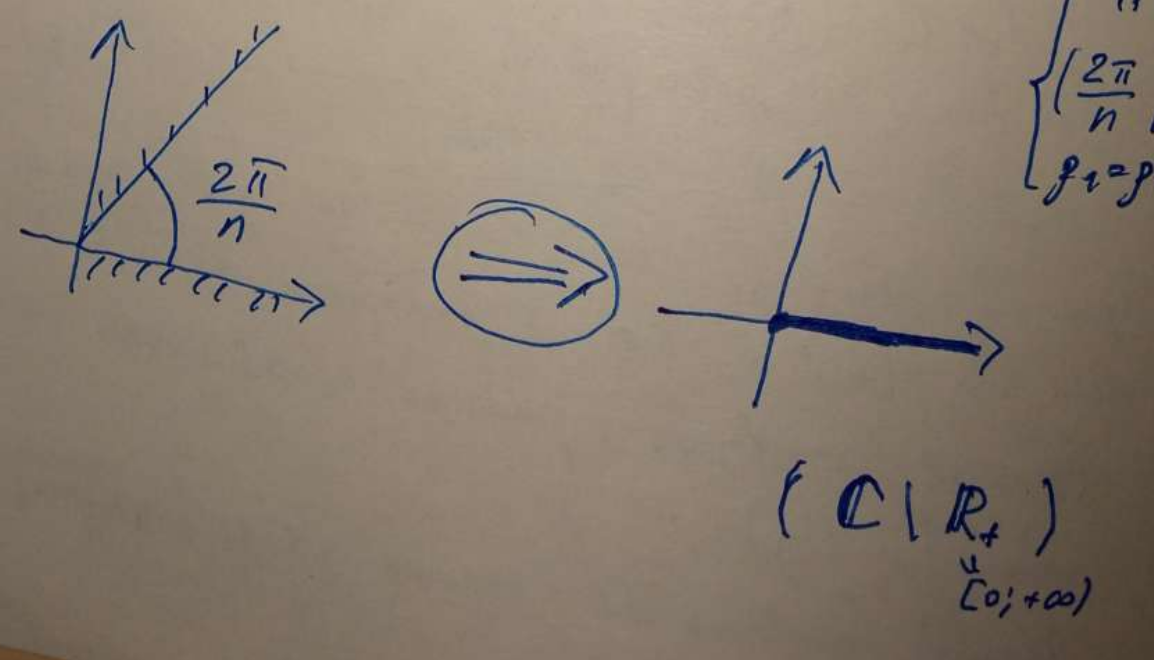
\includegraphics[scale=0.3]{assets/power_ex.png}
\end{example}

\begin{example}
	Рассмотрим $f = e^z$.

	Утверждается, что $f$ локально однолистна в $\mathbb{C}$, так как $f' = e^z \neq 0$.

	Причём
	\[
		e^{z_1} = e^{z_2} \Leftrightarrow e^{x_1}e^{iy_1} = e^{x_2}e^{iy_2} \Leftrightarrow \begin{cases}
			2\pi \:\vert\: y_1 - y_2 \\
			x_1 = x_2
		\end{cases}
	\]
	По аналогии, обратное отображение также конформно
	\[
		f^{-1}(w) = \ln\vert w\vert + i\arg(w),\, \arg(w) \in (0,\, 2\pi) \text{ - ветвь корня}
	\]

	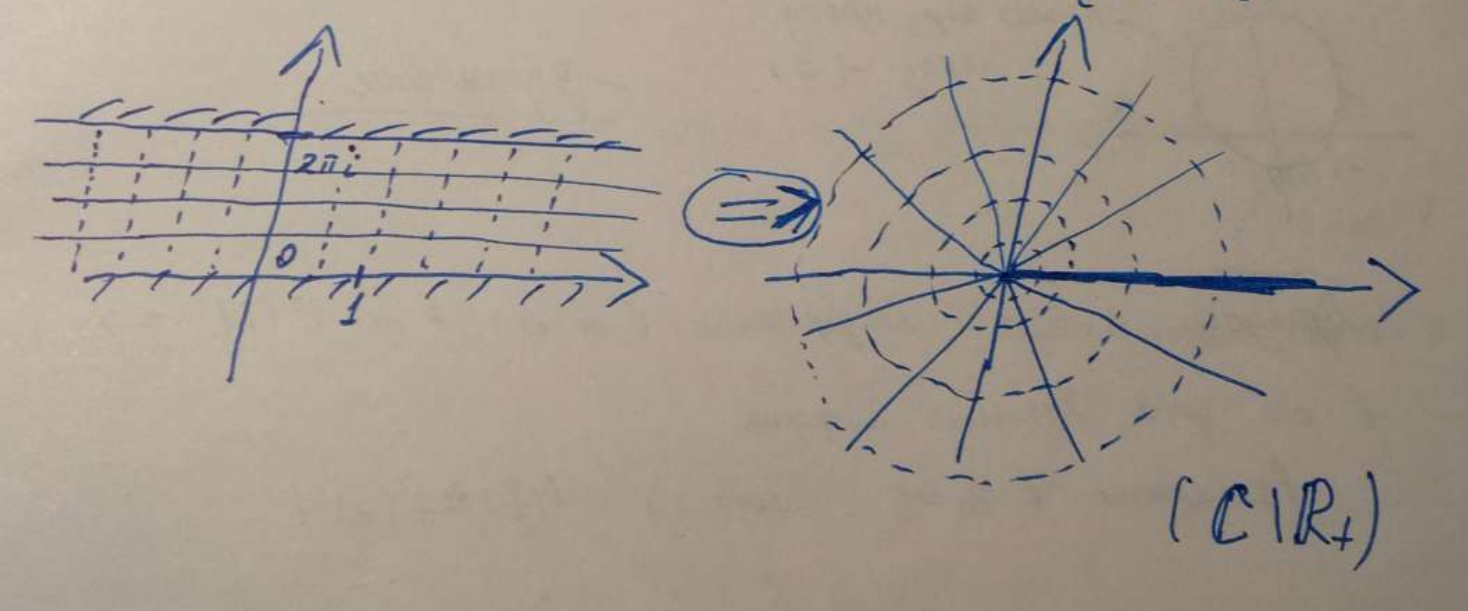
\includegraphics[scale=0.3]{assets/exp_ex.png}
\end{example}

\section{Локально равномерная сходимость и теоремы Вейерштрасса}
\begin{definition}
	Пусть $f_n$ определена в области $D$. Тогда $f_n$ локально равномерно сходится к $f$ в области $D$, если
	\[
		\forall z_0 \in D \: \exists \delta > 0 :\: O_\delta(z_0) \subset D :\: f_n \overset{O_\delta(z_0)}{\rightrightarrows} f
	\]
\end{definition}

\begin{proposition}
	Эквивалентное определение локально равномерной сходимости:
	\[
		\forall K \text{ - компакт}\subset D :\: f_n \overset{K}{\rightrightarrows} f
	\]
\end{proposition}

\begin{proof}
	($2 \Rightarrow 1$) В качестве компактов возьмём $\overline{O}_\delta(z_0)$

	($1 \Rightarrow 2$) Компакт покрываем шарами, выбираем конечное подпокрытие и получаем $\rightrightarrows$.
\end{proof}

\begin{theorem}
	Пусть $f_n$ голоморфны в $D$, $f_n$ сходится к $f$ локально равномерно в $D$. Тогда
	\begin{enumerate}
		\item $f$ -- голоморфна
		\item $f_n^{(k)}$ локально равномерно сходится к $f^{(k)}$ в $D$
	\end{enumerate}
\end{theorem}

\begin{proof}
	\begin{enumerate}
		\item По теореме Морера достаточно проверить непрерывность $f$ и
		      \[
			      \int_{\Gamma \text{ - замкнутой}}f(z)dz = 0
		      \]
		      Пусть $z_0 \in D,\, \overline{O}_r(z_0) \subset D$.

		      Используя определение с компактами получим, что $f_n \rightrightarrows f$ на $\overline{O}_r(z_0) \Rightarrow f$ непрерывна, как равномерный предел непрерывных.

		      Далее, пусть $\gamma$ -- кусочно гладкая кривая, замкнутая в $\overline{O}_r(z_0)$.

		      Так как
		      \[
			      \left\vert\int_\gamma (f_n - f)dz\right\vert \leq \int_\gamma\vert f_n - f\vert dz \leq \varepsilon_n\int_\gamma dz = c\varepsilon_n \overset{n \to \infty}{\to} 0
		      \]
		      поэтому
		      \[
			      \int_\gamma f_n(z)dz \to \int_\gamma f(z)dz
		      \]
		      Но
		      \[
			      \int_\gamma f_ndz = 0 \Rightarrow \int_\gamma f(z)dz = 0 \Rightarrow f \text{ - голоморфна}
		      \]
		\item Напишем формулу Коши

		      Пусть $z_0 \in D,\, O_r(z_0) \subset D,\, z \in O_{\frac{r}{2}}(z_0)$. Тогда
		      \[
			      f'(z) = \frac{1}{2\pi i} \int_{\partial O_r(z_0)}\frac{f(\xi)d\xi}{(\xi - z)^2};\;\;\;\; f_n'(z) = \frac{1}{2\pi i}\int_{\partial O_r(z_0)}\frac{f_n(\xi)d\xi}{(\xi - z)^2}
		      \]
		      Тогда
		      \begin{align*}
			      \vert f'(z) - f_n'(z)\vert \leq \left\vert\frac{1}{2\pi i}\int_{\gamma_r}\frac{\vert f(\xi) - f_n(\xi)\vert\vert d\xi\vert}{\vert \xi - z\vert^2}\right\vert \leq \\
			      \frac{1}{2\pi}\max_{\gamma_r}\vert f- f_n\vert\cdot\left\vert\int_{\gamma_r}\frac{\vert d\xi\vert}{\vert \xi - z\vert^2}\right\vert \leq \frac{2}{\pi r^2}\max_{\gamma_r}\vert f - f_n\vert\cdot2\pi r = c\max_{\gamma_r}\vert f - f_n\vert \to 0
		      \end{align*}
		      При этом $c = \frac{4}{r} \Rightarrow$ стремление на самом деле равномерное на $O_{\frac{r}{2}}(z_0)$. Так можно сделать $\forall z_0 \Rightarrow$ по первому определению $f'$ локально равномерно сходится к $f$ в $D$. Дальше -- очев индукция.
	\end{enumerate}
\end{proof}

\begin{theorem}
	Пусть $f_n$ голоморфна в $D,\, \sum_{n = 1}^\infty f_n$ локально равномерно сходится в области $D$. Тогда
	\begin{enumerate}
		\item $f := \sum_{n = 1}^\infty f_n$ -- голоморфная функция
		\item $f' = \sum_{n = 1}^\infty f_n'$
	\end{enumerate}
\end{theorem}

\begin{proof}
	$\tilde{f}_k := \sum_{n = 1}^k f_n$ и применяем теорему Вейерштрасса.
\end{proof}

\end{document}
